\RequirePackage{luatex85}
\documentclass[handout]{beamer}
\setbeamertemplate{caption}[numbered]
\usepackage{textpos}
\usepackage{listings}
\usepackage{graphicx}
\usepackage{xcolor}

\usepackage{tikz}
\usetikzlibrary{arrows}
\usetikzlibrary{graphs}
\usetikzlibrary{graphdrawing}
\usegdlibrary{force}
\usegdlibrary{layered}
\usegdlibrary{trees}

\usepackage{csquotes}


\usepackage{xcolor}
\definecolor{mygreen}{rgb}{0,0.6,0}
\definecolor{mygray}{rgb}{0.5,0.5,0.5}

\newcommand\Wider[2][3em]{%
\makebox[\linewidth][c]{%
  \begin{minipage}{\dimexpr\textwidth+#1\relax}
  \raggedright#2
  \end{minipage}%
  }%
}

\lstset{language=C++,
           basicstyle=\ttfamily\scriptsize,
           keywordstyle=\color{blue}\ttfamily,
           stringstyle=\color{red}\ttfamily,
           commentstyle=\color{mygreen}\ttfamily,
          breaklines=true,
          captionpos=b,
          numbers=left,
          numbersep=5pt,
          numberstyle=\tiny\color{mygray},
          rulecolor=\color{black},
          xleftmargin=\parindent,
          frame=single,
          backgroundcolor=\color{white}
}

% \usepackage{beamerthemesplit} // Activate for custom appearance
%\usecolortheme{whale}
\setbeamercolor{normal text}{fg=black,bg=white}
\definecolor{beamer@blendedblue}{rgb}{0,0,0}
\setbeamercolor{structure}{fg=beamer@blendedblue}


\title{Introduction to Object Detection \\ \& Image Segmentation}
\author{
	
\includegraphics[width=3cm]{../media/logo/NVLogo_2D.eps}
	\vspace{0.75cm}
	\\Abel Brown}
\date{\today}

\begin{document}

\frame{\titlepage}

%\section[Outline]{}
\begin{frame}{Outline}
\tableofcontents
\end{frame}


\addtobeamertemplate{frametitle}{}{%
\begin{textblock*}{200mm}(.75\textwidth,-0.35cm)

\includegraphics[width=3cm]{../media/logo/NVLogo_2D_H.eps}
\end{textblock*}}

\addtobeamertemplate{navigation symbols}{}{%
    \usebeamerfont{footline}%
    \usebeamercolor[fg]{footline}%
    \hspace{1em}%
    \insertframenumber/\inserttotalframenumber
}

%\section{Introduction}
%\subsection{Overview of the Beamer Class}

%\frame
%{
 %\frametitle{What is CUDA?}
%
%  \begin{itemize}
%  \item<1-> Normal LaTeX class.
%  \item<2-> Easy overlays.
%  \item<3-> No external programs needed.      
%  \end{itemize}
%}

\section{What is Object Detection and Segmentation?}
\begin{frame}{What is Object Detection?}
\emph{Object detection is a computer technology related to computer vision and image processing that deals with detecting instances of semantic objects of a certain class (such as humans, buildings, or cars) in digital images and videos.}. \footnote{\href{https://en.wikipedia.org/wiki/Object_detection}{\color{blue}Wikipedia}}
\end{frame}

\begin{frame}{What is Image Segmentation?}
\emph{In computer vision, image segmentation is the process of partitioning a digital image into multiple segments (sets of pixels, also known as super-pixels). The goal of segmentation is to simplify and/or change the representation of an image into something that is more meaningful and easier to analyze.  Image segmentation is typically used to locate objects and boundaries (lines, curves, etc.) in images}. \footnote{\href{https://en.wikipedia.org/wiki/Image_segmentation}{\color{blue}Wikipedia}}
\end{frame}

\begin{frame}{What is Image Segmentation?}
\emph{More precisely, image segmentation is the process of assigning a label to every pixel in an image such that pixels with the same label share certain characteristics}.\footnote{\href{https://en.wikipedia.org/wiki/Image_segmentation}{\color{blue}Wikipedia}}
\end{frame}

\begin{frame}{Generic Detection and Segmentation}
Given an input tensor of size $CxHxW$ constructed from pixel values of some image ...
\begin{itemize}
  \item<1->\emph{identify} content of interest
  \item<2->\emph{locate} the interesting content 
  \item<3->\emph{partition} input (i.e. pixels) corresponding to identified content
 \\~\\ 
 \begin{tabular}{cccc}
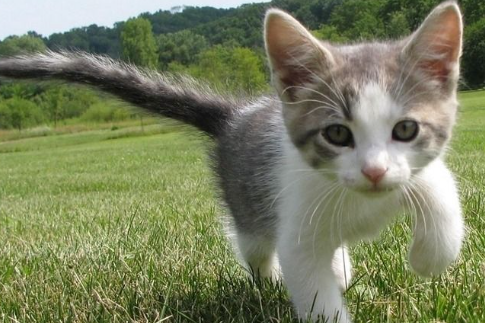
\includegraphics[width=0.2\textwidth]{../media/cat1} &
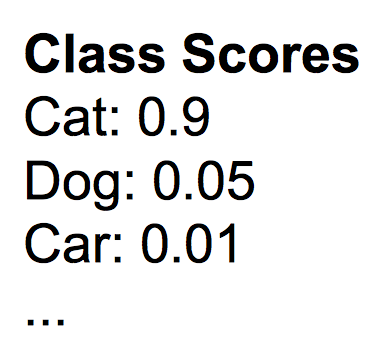
\includegraphics[width=0.2\textwidth]{../media/cat2} &
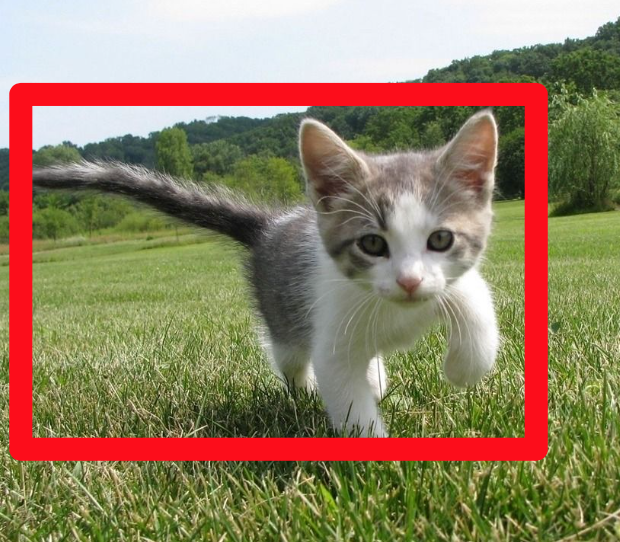
\includegraphics[width=0.2\textwidth]{../media/cat3} & 
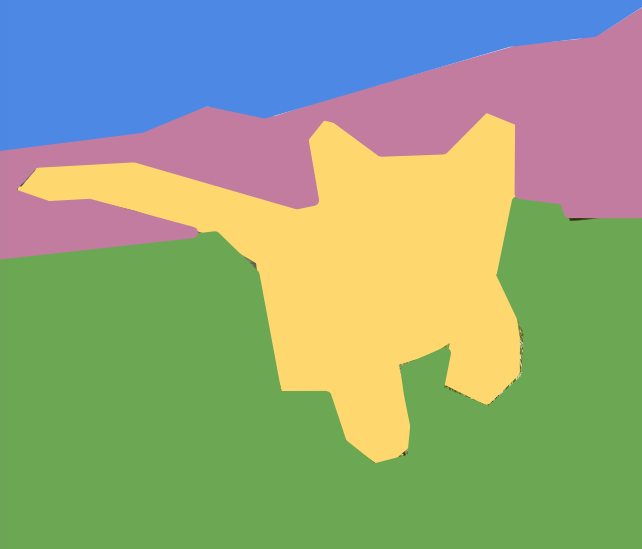
\includegraphics[width=0.2\textwidth]{../media/cat4}
\end{tabular}\footnote{\href{http://cs231n.stanford.edu/slides/2017/cs231n_2017_lecture11.pdf}{\color{blue}Stanford cs231n (2017)}}
\\~\\
\item<4->Workflow: object detection, localization, and segmentation 
\end{itemize}
\end{frame}

\section{Examples} 

\begin{frame}{Examples: Binary Mask}
\begin{figure}
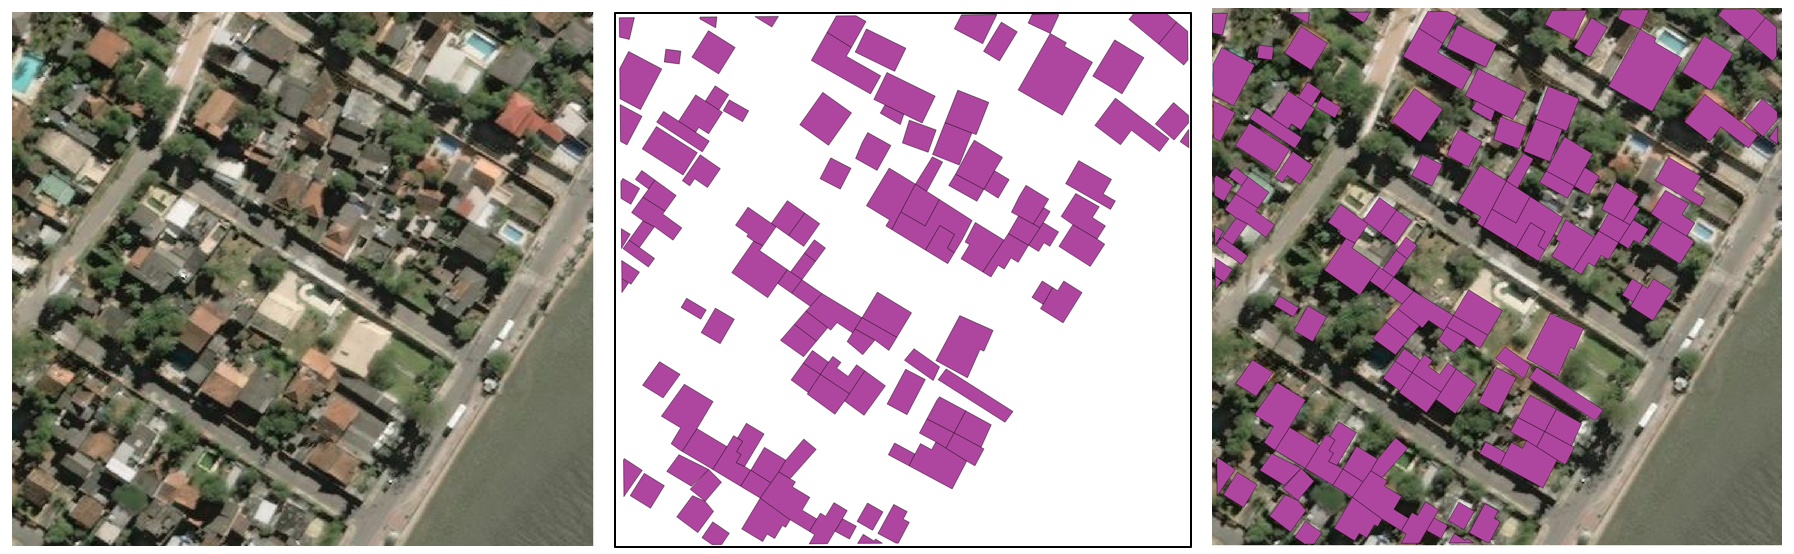
\includegraphics[width=\textwidth]{../media/spacenet_1.png}
\caption{\href{https://devblogs.nvidia.com/parallelforall/exploring-spacenet-dataset-using-digits}{\color{blue} SpaceNet sample data}}
\end{figure}
\end{frame}

\begin{frame}{Examples: Binary Mask}
\begin{figure}
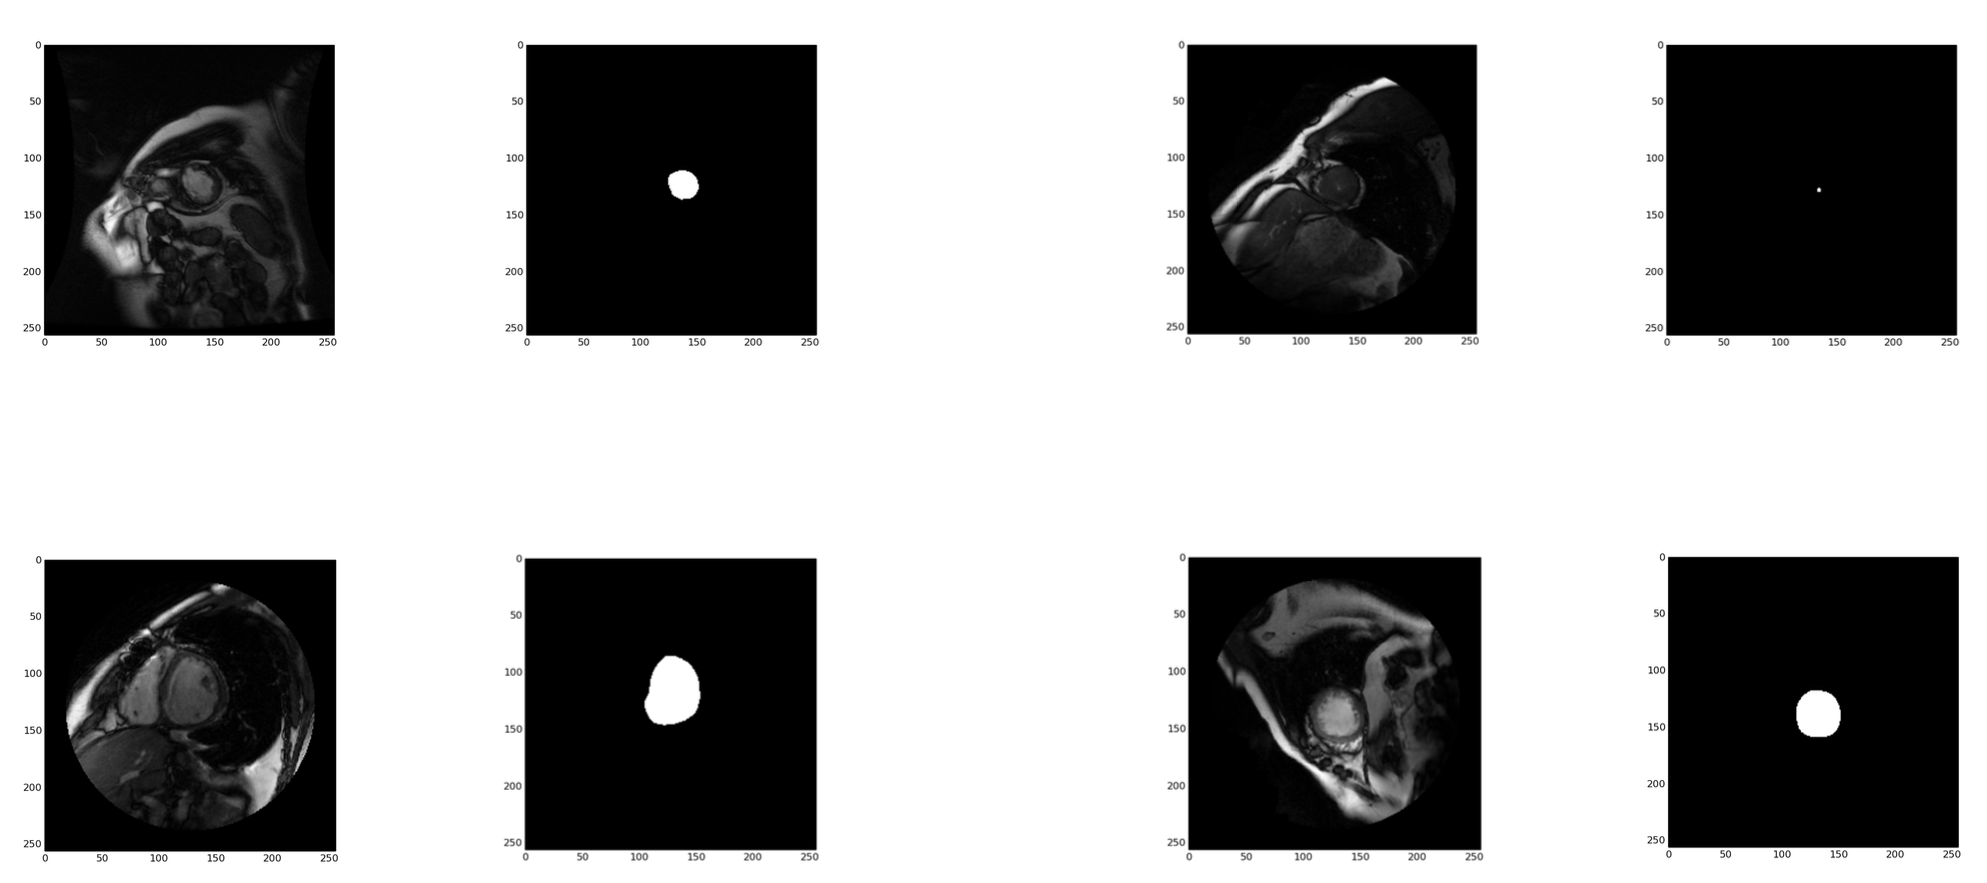
\includegraphics[width=\textwidth]{../media/lv_segmentation.png}
\caption{\href{http://www.cardiacatlas.org/studies/sunnybrook-cardiac-data/}{\color{blue} Sunnybrook - Left ventricle segmentation} (fMRI)}
\end{figure}
\end{frame}

\begin{frame}{Examples: Binary Mask}
\begin{figure}
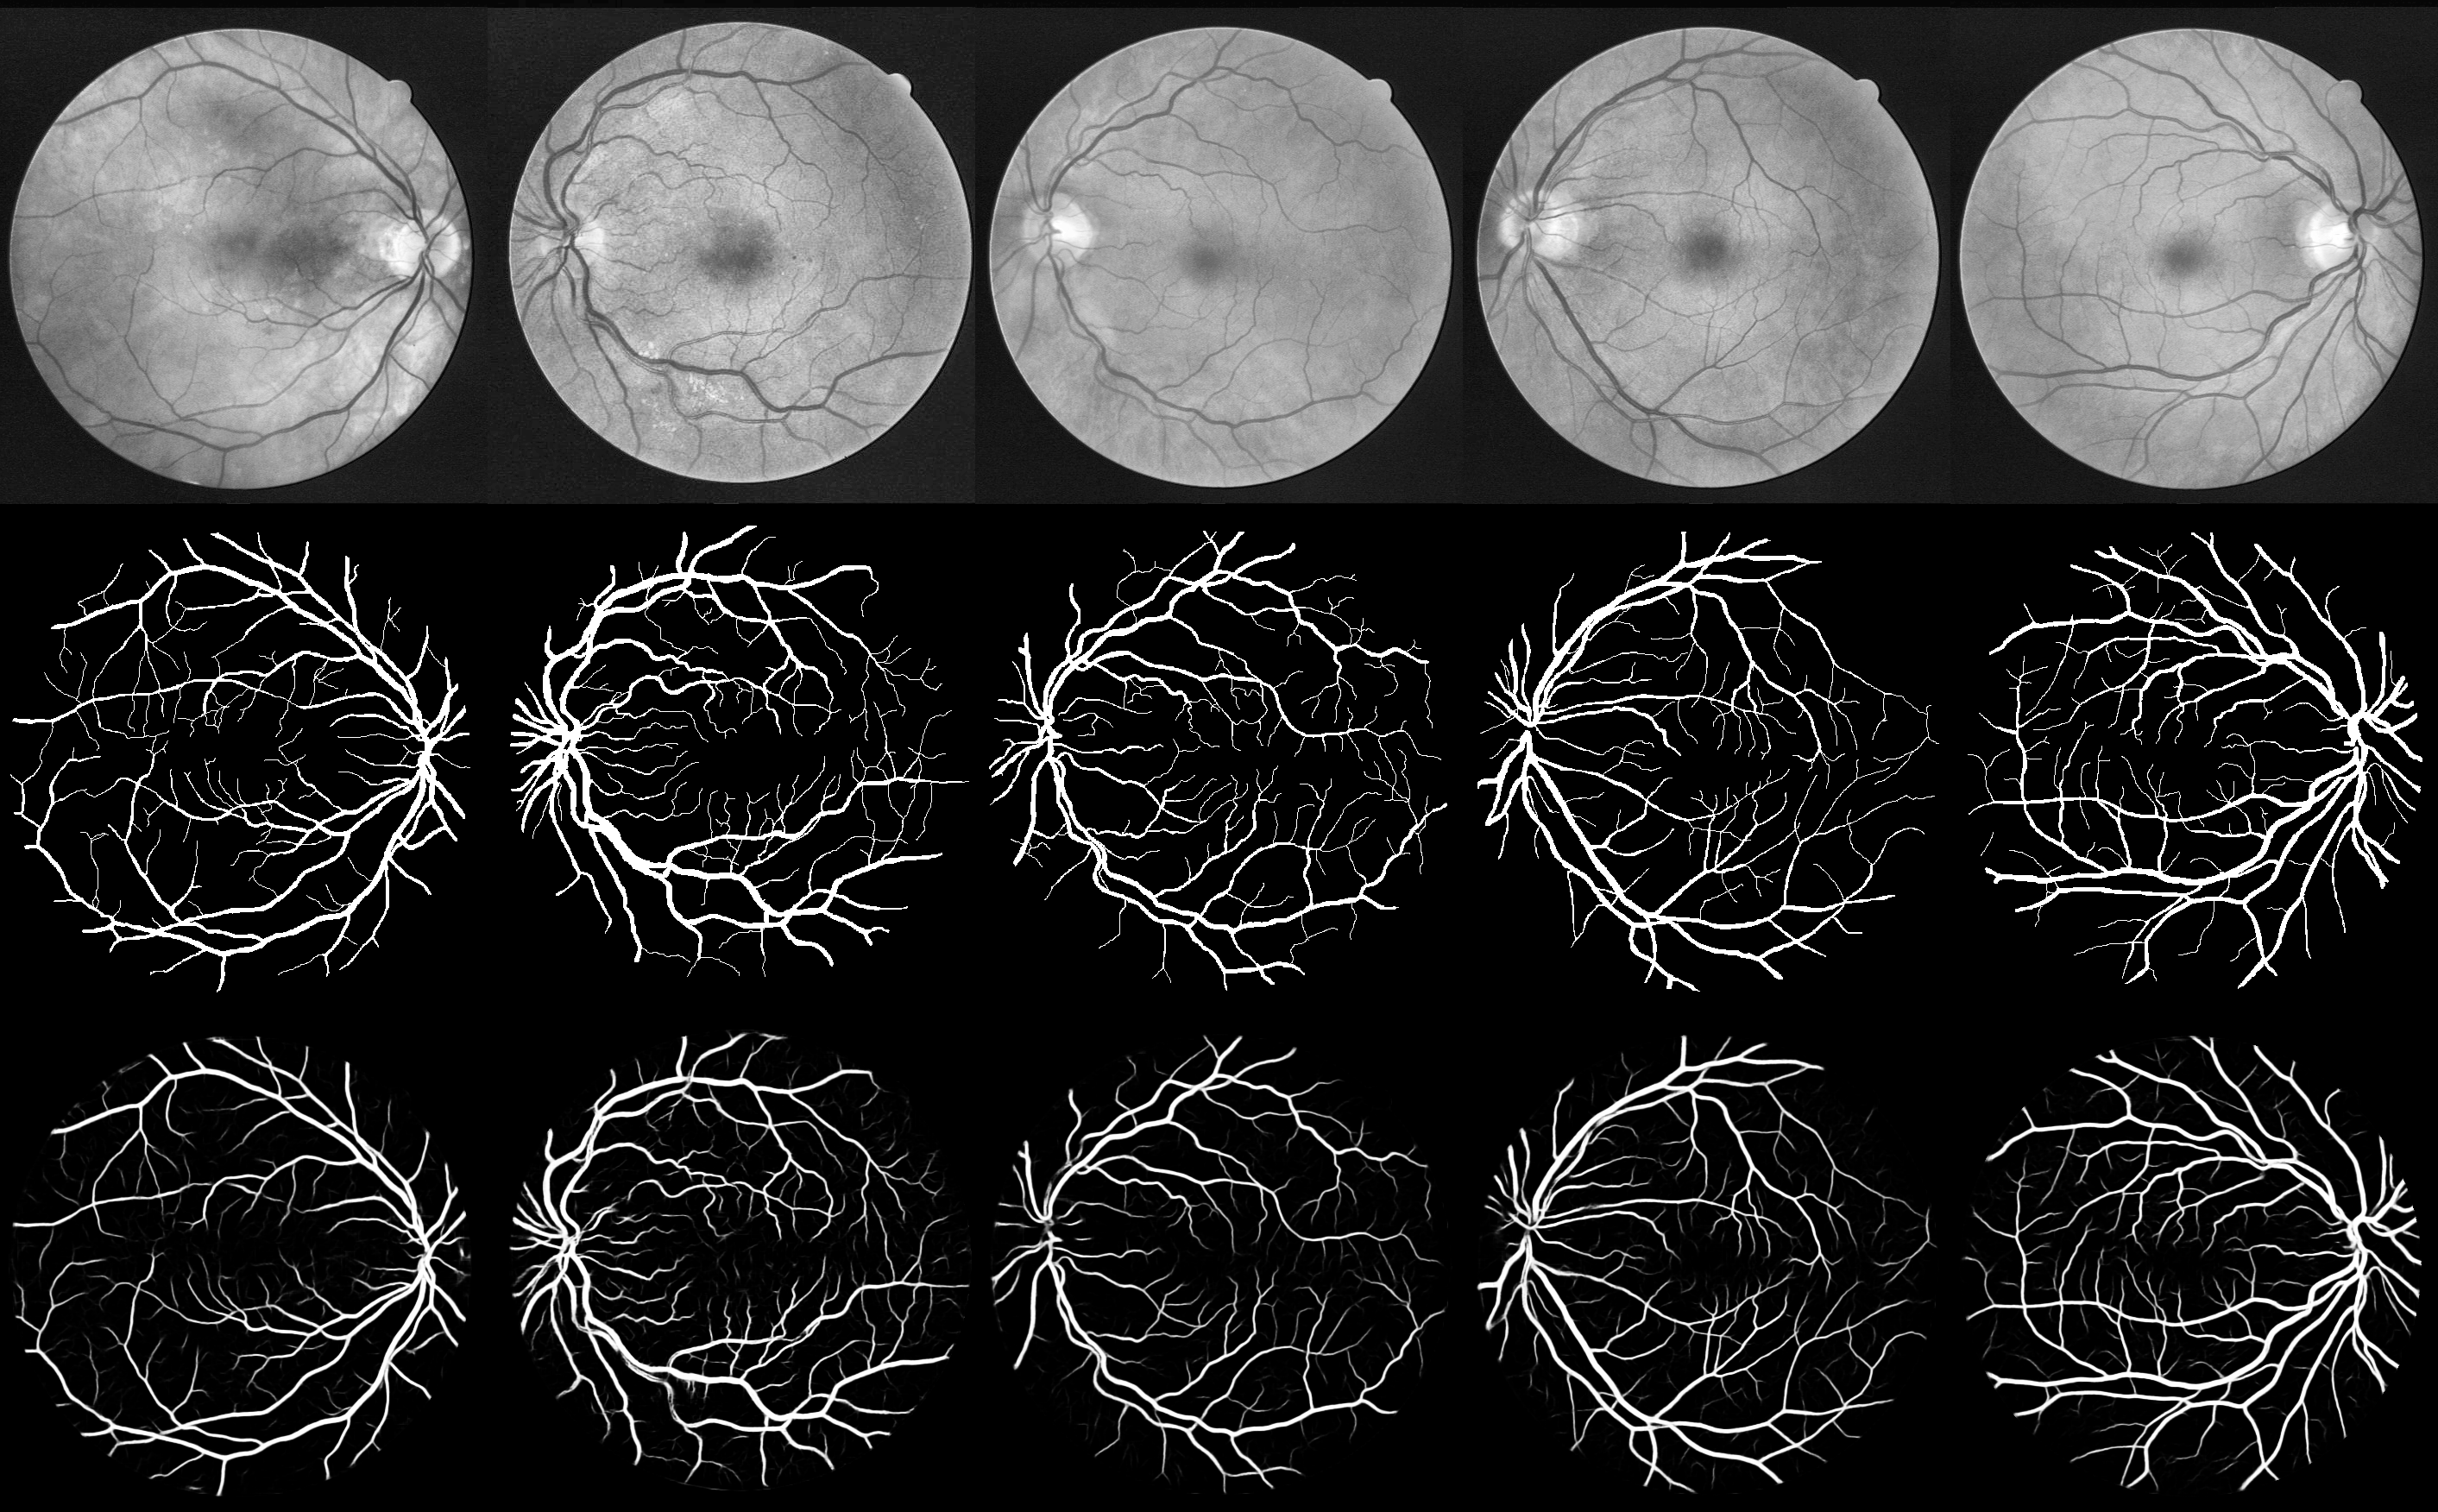
\includegraphics[width=0.8\textwidth]{../media/unet_retina_segmentation.png}
\caption{\href{https://github.com/orobix/retina-unet}{\color{blue} U-Net: CNNs for Biomedical Image Segmentation}}
\end{figure}
\end{frame}

\begin{frame}{Examples: Multiclass}
\begin{figure}
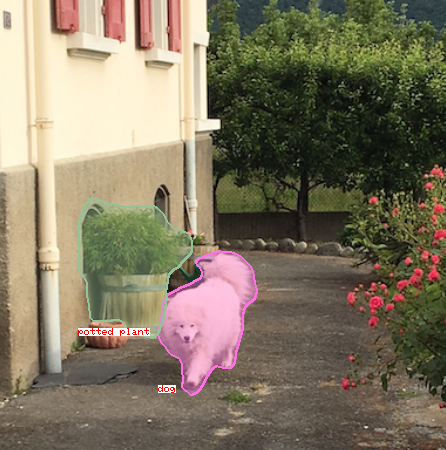
\includegraphics[width=0.6\textwidth,keepaspectratio]{../media/multipath_network_2.png}
\caption{\href{https://research.fb.com/learning-to-segment/}{\color{blue}FAIR: Learning to Segment}}
\end{figure}
\end{frame}

\begin{frame}{Examples (and More Lingo)}
\begin{figure}
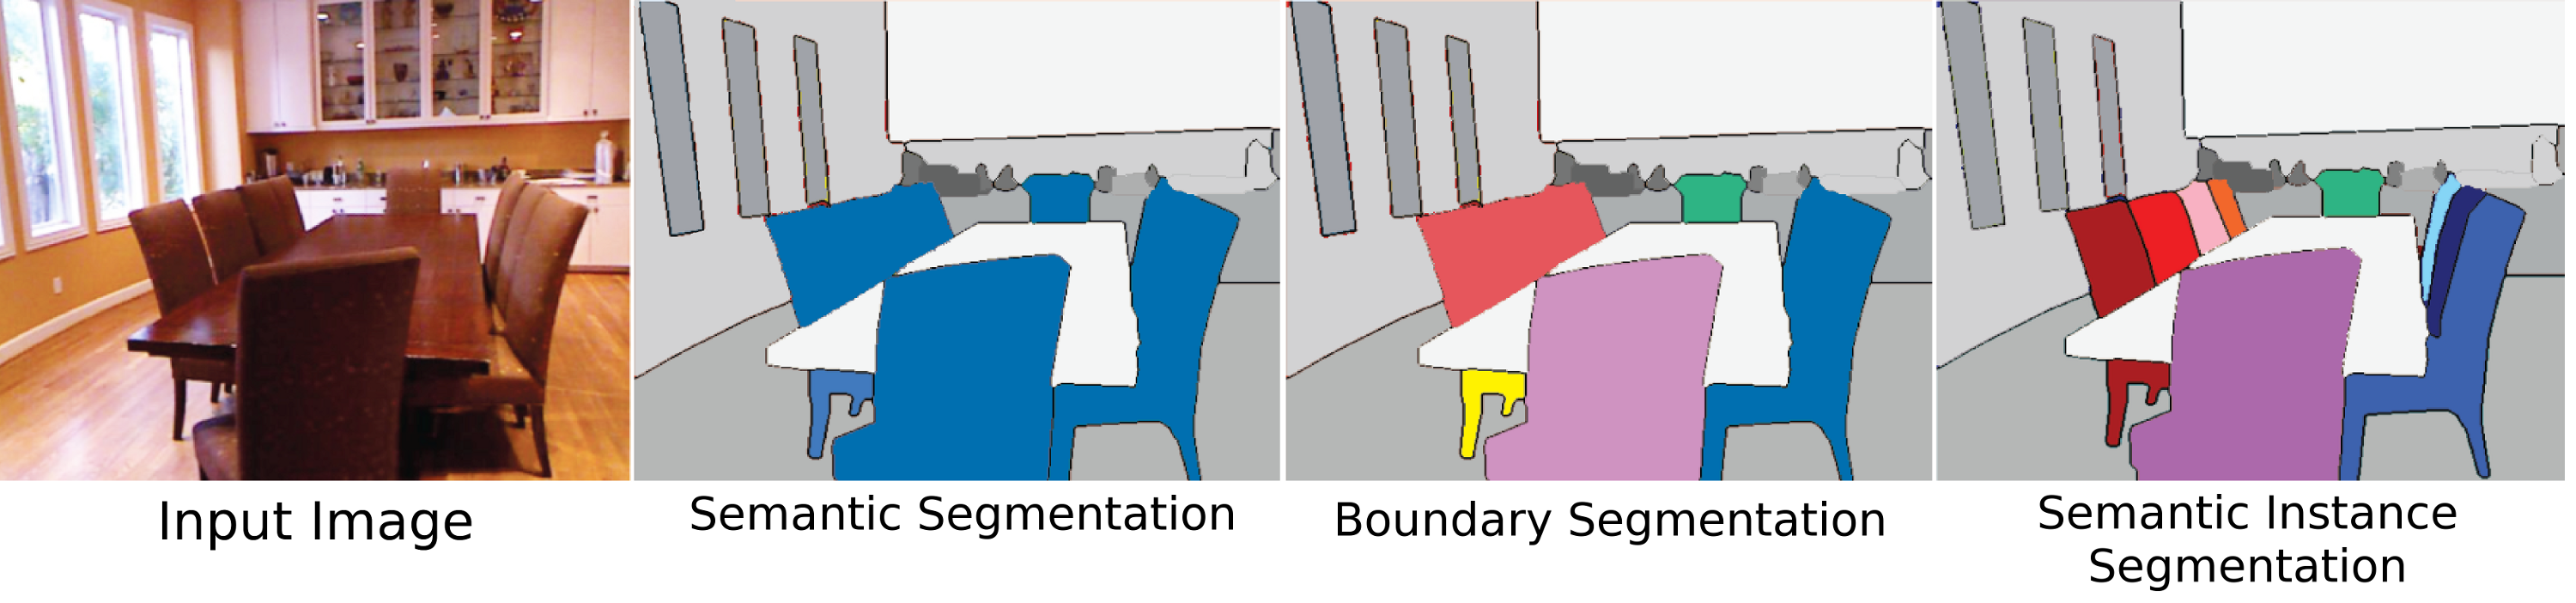
\includegraphics[width=\textwidth]{../media/instance_segmentation_nyu.png}
\caption{\href{http://cs.nyu.edu/~silberman/projects/instance_segmentation.html}{\color{blue} Silberman - Instance Segmentation}}
\end{figure}
\end{frame}

\begin{frame}{Boundary Segmentation Examples}
\begin{figure}
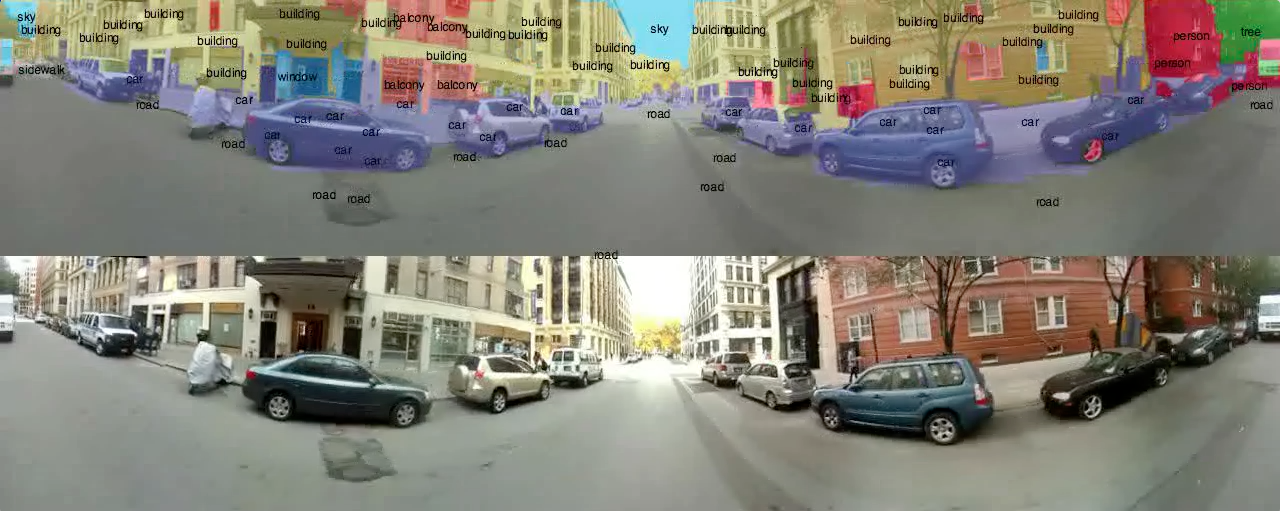
\includegraphics[width=\textwidth]{../media/park-nyu-1-parsed.png}
\caption{\href{http://www.clement.farabet.net/research.html\#parsing}{\color{blue} Farabet - Scene Parsing}}
\end{figure}
\end{frame}

\begin{frame}{Boundary Segmentation Examples}
\begin{figure}
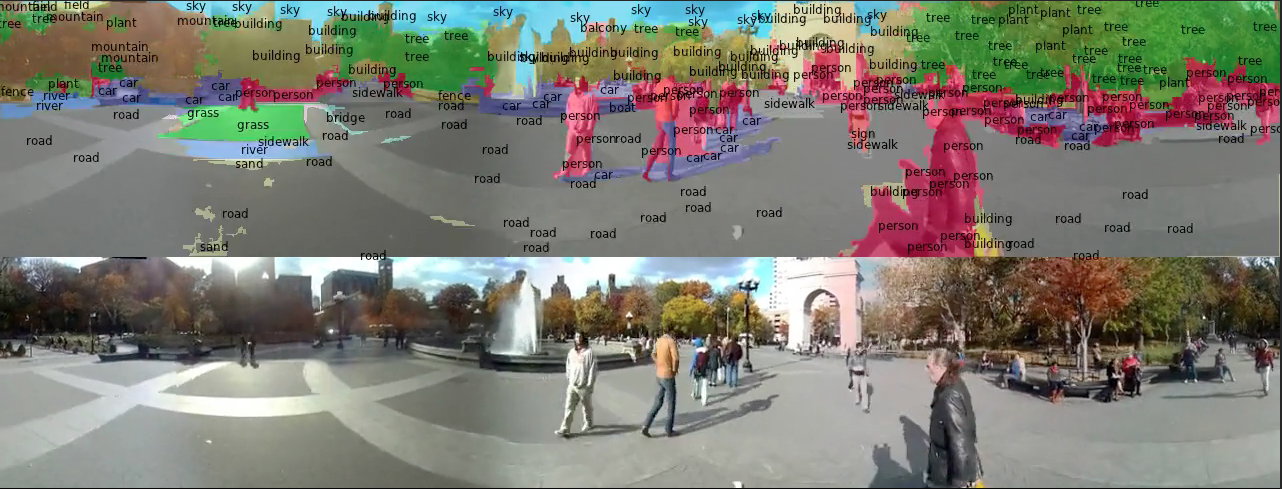
\includegraphics[width=\textwidth]{../media/park-nyu-2-parsed.png}
\caption{\href{http://www.clement.farabet.net/research.html\#parsing}{\color{blue} Farabet - Scene Parsing}}
\end{figure}
\end{frame}

%\begin{frame}{Instance Segmentation Examples}
%\begin{figure}
%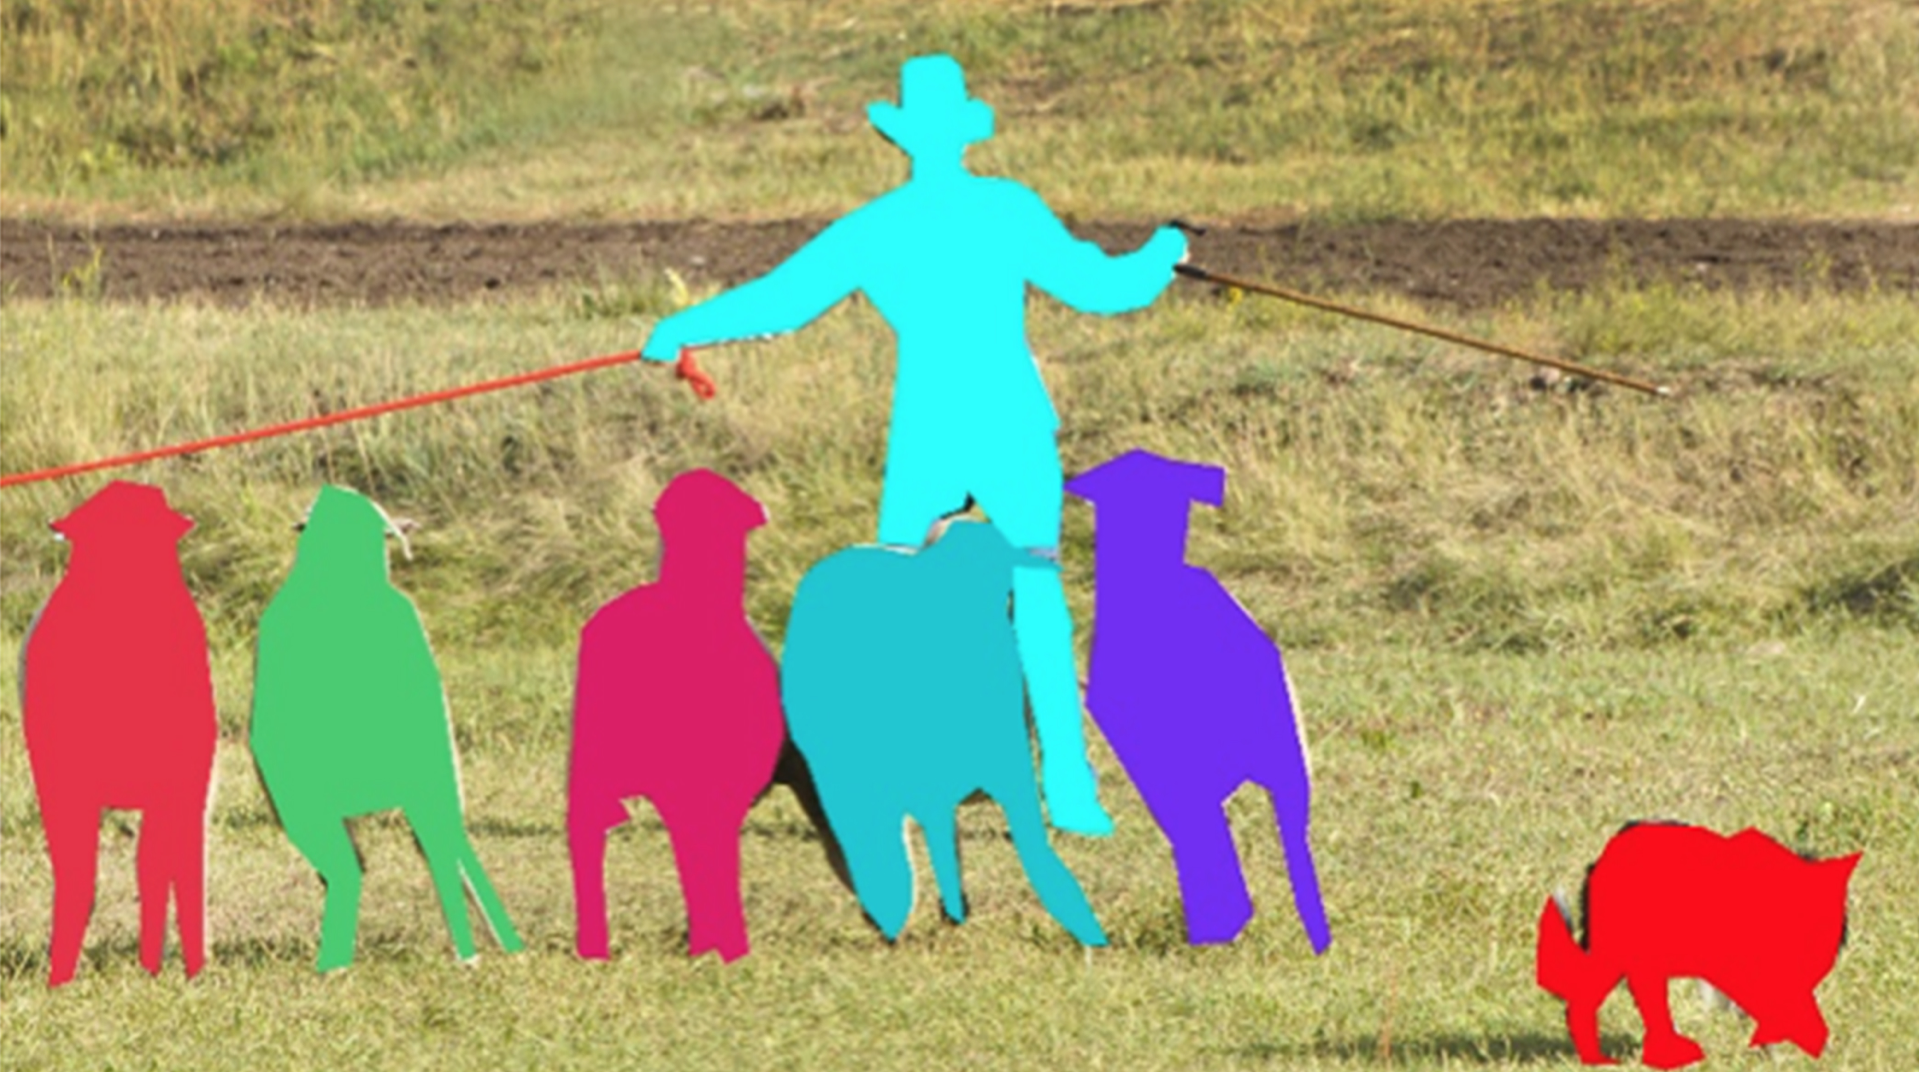
\includegraphics[width=\textwidth]{../media/multipath_network_6.png}
%\caption{\href{https://research.fb.com/learning-to-segment/}{\color{blue}FAIR: Learning to Segment}}
%\end{figure}
%\end{frame}

\begin{frame}{Instance Segmentation Examples}
\begin{figure}
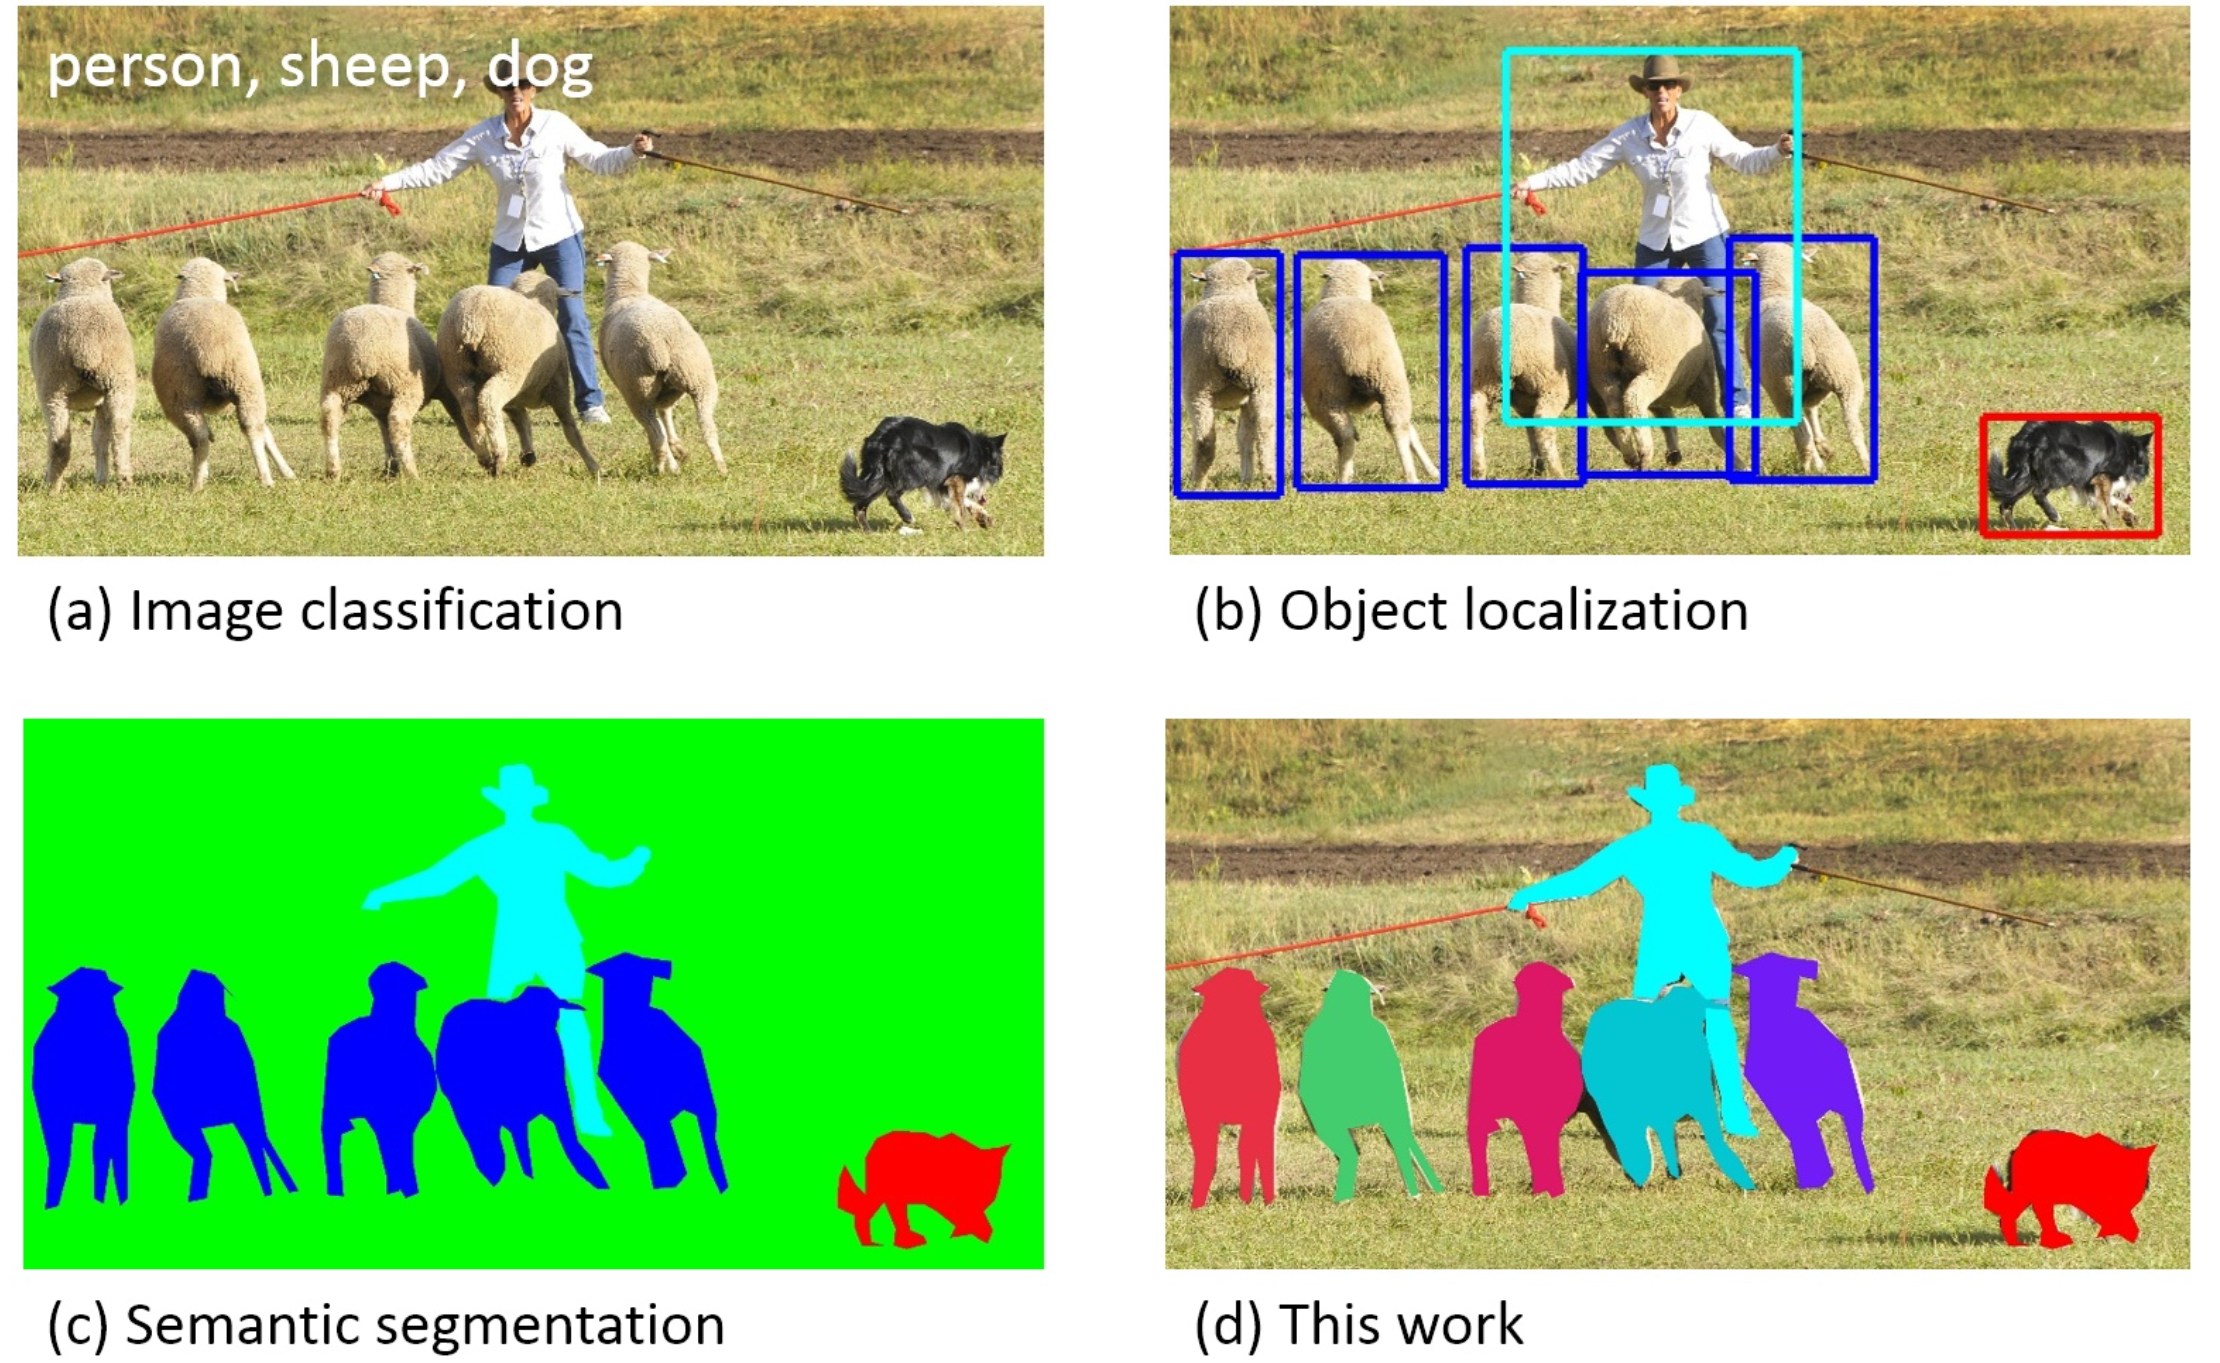
\includegraphics[width=\textwidth]{../media/coco_1.png}
\caption{\href{https://research.fb.com/learning-to-segment/}{\color{blue}Microsoft COCO: Common Objects in Context}}
\end{figure}
\end{frame}


\begin{frame}{Instance Segmentation Examples}
\begin{figure}
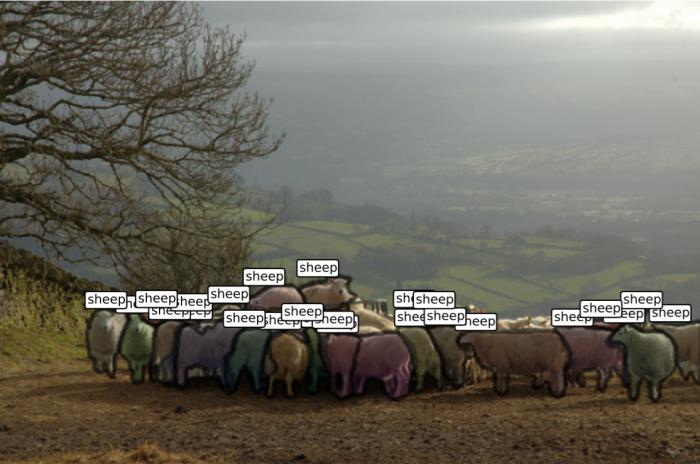
\includegraphics[width=0.9\textwidth,keepaspectratio]{../media/multipath_network_1.jpg}
\caption{\href{https://arxiv.org/abs/1405.0312v3}{\color{blue}FAIR: A MultiPath Network for Object Detection}}
\end{figure}
\end{frame}


\begin{frame}{Image Segmentation Examples}
\begin{figure}
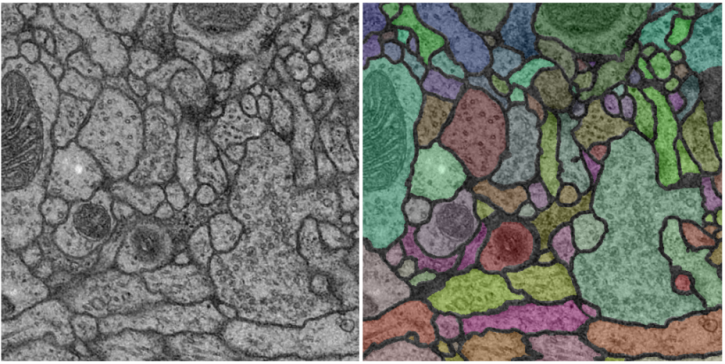
\includegraphics[width=0.9\textwidth,keepaspectratio]{../media/neuronal_segmentation.png}
\caption{\href{https://papers.nips.cc/paper/4741-deep-neural-networks-segment-neuronal-membranes-in-electron-microscopy-images}{\color{blue}Ciresan - Neuronal membrane segmentation}}
\end{figure}
\end{frame}

\begin{frame}{Image Segmentation Examples}
\begin{figure}
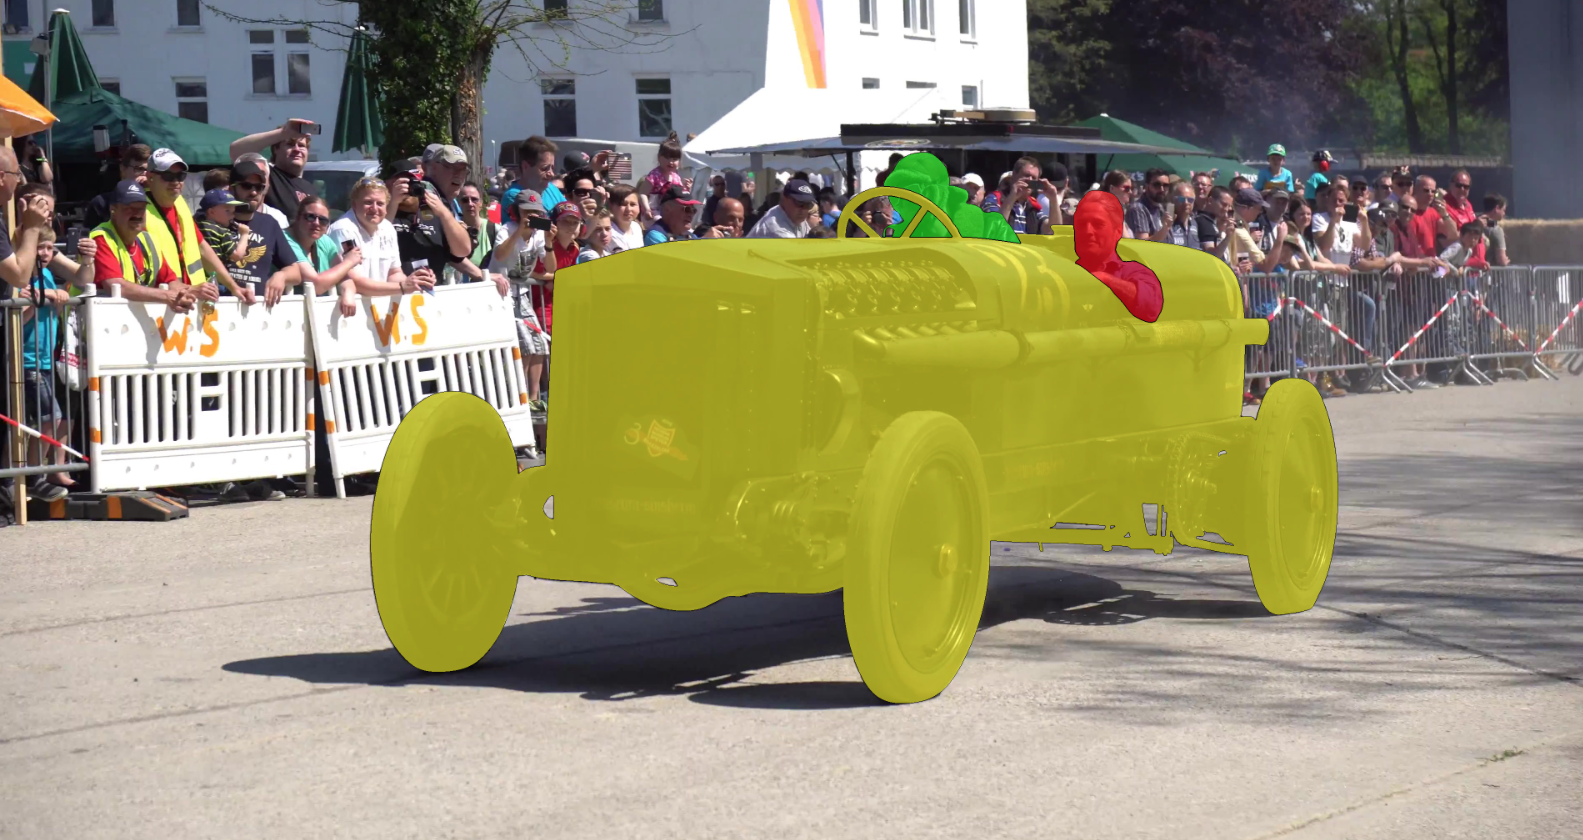
\includegraphics[width=\textwidth]{../media/davis_1.png}
\caption{\href{http://davischallenge.org/index.html}{\color{blue}DAVIS: Densely Annotated VIdeo Segmentation}}
\end{figure}
\end{frame}

\section{Before Deep Learning}  

\begin{frame}{History: Pre Deep Learning}
\begin{itemize}
  \item<1-> Object detection, localization, and segmentation has a long history before deep learning became popular
  \item<2-> Years before \href{http://www.image-net.org}{\color{blue}ImageNet}\footnote{\href{http://www.image-net.org/papers/imagenet_cvpr09.pdf}{\color{blue}ImageNet: A Large-Scale Hierarchical Image Database}} and deep learning there was \href{http://host.robots.ox.ac.uk/pascal/VOC/}{\color{blue}PASCAL}\footnote{\href{http://host.robots.ox.ac.uk/pascal/VOC/pubs/everingham10.html\#abstract}{\color{blue}The PASCAL Visual Object Classes (VOC) Challenge}}\textsuperscript{,}\footnote{\href{http://host.robots.ox.ac.uk/pascal/VOC/pubs/everingham15.html\#abstract}{\color{blue}The PASCAL Challenge: A Retrospective}} and custom computer vision techniques
  \item<3-> Many early algorithms shared similar structure:
  \begin{itemize}
  	\item<1->identify potentially relevant content (region proposals)
	\item<2->for each proposed region, test/label region 
	\item<3->aggregate results from all regions to form final answer/result/output for the image
  \end{itemize}
  \item<4->Even early DL based algorithms shared this structure (Overfeat, R-CNN, etc)
  \item<5->Recently, some successful \emph{single-stage} DL approaches 
\end{itemize}
\end{frame}

\begin{frame}{Pre Deep Learning Methods}
\begin{tabular}{lcc}
	\href{http://www.vision.caltech.edu/CNS179/papers/Poggio98.pdf}{\color{blue}Example-Based Learning} \dotfill&1998 & 2435 \\
	\href{http://fcv2011.ulsan.ac.kr/files/announcement/413/IJCV(2004)\%20Efficient\%20Graph-Based\%20Image\%20Segmentation.pdf}{\color{blue}Efficient Graph-Based Image Segmentation} \dotfill& 2004 & 4787 \\
	\href{www.robots.ox.ac.uk/~vgg/research/affine/det_eval_files/lowe_ijcv2004.pdf}{\color{blue}Image Features from Scale-Invariant Keypoints} \dotfill  & 2004 & 42365 \\
	\href{https://hal.inria.fr/file/index/docid/548512/filename/hog_cvpr2005.pdf}{\color{blue}Histograms of Oriented Gradients} \dotfill& 2005 & 19435 \\
	\href{http://dhoiem.web.engr.illinois.edu/publications/eccv2010_CategoryIndependentProposals_ian.pdf}{\color{blue}Category Independent Object Proposals} \dotfill& 2010 & 367 \\
	\href{https://pdfs.semanticscholar.org/648a/ccff91feda12ece4cdbde713bb3f7fc54045.pdf}{\color{blue}Constrained Parametric Min-Cuts} \dotfill & 2010 & 387 \\
	\href{https://cs.brown.edu/~pff/papers/lsvm-pami.pdf}{\color{blue}Discriminatively Trained Part Based Models} \dotfill& 2010 & 5646 \\
	\href{http://ai2-s2-pdfs.s3.amazonaws.com/b967/9890b45ddc60234a158eb83926c5a392bd4a.pdf}{\color{blue}Measuring the objectness of image windows} \dotfill & 2011 & 669 \\
	\href{https://ivi.fnwi.uva.nl/isis/publications/bibtexbrowser.php?key=UijlingsIJCV2013\&bib=all.bib}{\color{blue}Selective Search for Object Recognition}\dotfill & 2012 & 1212 \\
	\href{http://www.ece.northwestern.edu/~mya671/mypapers/ICCV13_Wang_Yang_Zhu_Lin.pdf}{\color{blue}Regionlets for Generic Object Detection} \dotfill & 2013 & 218 \\
	\href{http://www.cv-foundation.org/openaccess/content_cvpr_2014/papers/Arbelaez_Multiscale_Combinatorial_Grouping_2014_CVPR_paper.pdf}{\color{blue}Multiscale Combinatorial Grouping} \dotfill & 2014 & 468 \\
\end{tabular}
\end{frame}

\section{Common Issues with Algorithms}
\begin{frame}{Common Issues with Algorithms}
\begin{itemize}
\itemsep1em
	\item<1->Compute performance often poor 
		\begin{itemize}\setbeamertemplate{itemize items}[square]
			\item<1->Too many region proposals to test and label
			\item<2->Difficult to scale to larger image size and/or frame rate
			\item<3->Cascading approaches help but not solve
			\item<4->Aggressive region proposal suppression leads to accuracy issues
		\end{itemize}
	\item<2->Accuracy problems
		\begin{itemize}\setbeamertemplate{itemize items}[square]
			\item<1->Huge number of candidate regions inflates false-positive rates
			\item<2->Illumination, occlusion, etc. can confuse test and label process
		\end{itemize}
	\item<3->Not really scale invariant
		\begin{itemize}\setbeamertemplate{itemize items}[square]
			\item<1->Early datasets not very large so limited feature variation
			\item<2->Now training datasets are many TB -- helps but does not solve
			\item<3->Large variation of feature scale can inflate false-negative rates
		\end{itemize}
\end{itemize}
\end{frame}

\section{Quality Assessment and Comparison Metrics}
\begin{frame}{Quality Assessment and Metrics}
\begin{itemize}
\itemsep 1.25em
	\item<1->Assessing the quality of a classification result is generally well defined
	\item<2->Quality assessment of object localization and segmentation results is more complex
	\begin{itemize}\setbeamertemplate{itemize items}[square]
		\item<1->\underline{Object localization} output is bounding box
		\item<2->How to assess overlap between ground truth and computed bounding boxes?
		\item<3->What about \emph{sloppy} or \emph{loose} ground truth bounding boxes?
	\end{itemize}
	
	\begin{itemize}\setbeamertemplate{itemize items}[square]
		\item<4->\underline{Segmentation} output is polygon-like pixel region
		\item<5->How to assess overlap of polygon-like ground truth and computed output region?
		\item<6->What about \emph{sloppy} or \emph{corse} ground truth regions?
	\end{itemize}
	\item<3->All this gets a bit more complicated when considering video (i.e. continuous stream of highly correlated images)
\end{itemize}
\end{frame}

\begin{frame}{Quality Assessment and Metrics}
Good, great, not bad, terrible?
\begin{figure}
\centering
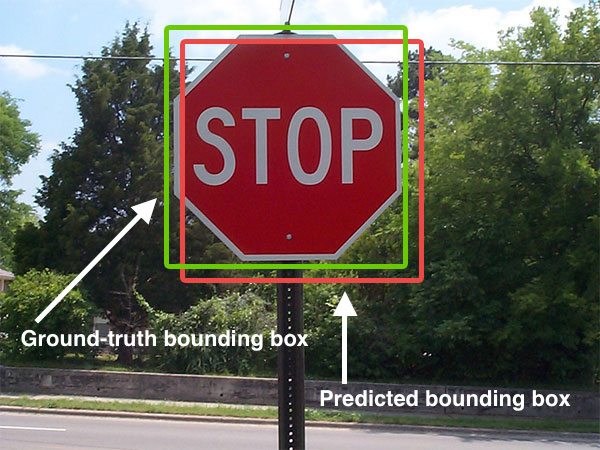
\includegraphics[width=0.8\textwidth]{../media/iou_stop_sign.jpg}
\caption{\href{http://www.pyimagesearch.com/2016/11/07/intersection-over-union-iou-for-object-detection/}{\color{blue}pyimagesearch.com}}
\end{figure}
\end{frame}


\begin{frame}{Quality Assessment and Metrics}
Good, great, not bad, terrible?
\begin{figure}
\centering
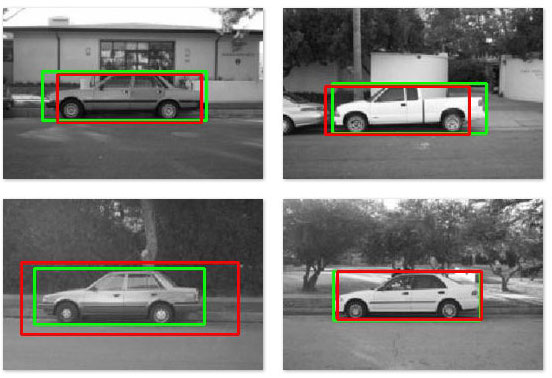
\includegraphics[width=0.9\textwidth]{../media/iou_car_bbs.jpg}
\caption{\href{http://www.pyimagesearch.com/2016/11/07/intersection-over-union-iou-for-object-detection/}{\color{blue}pyimagesearch.com}}
\end{figure}
\end{frame}

\begin{frame}{Quality Assessment and Metrics}
Good, great, not bad, terrible?
\begin{figure}
\centering
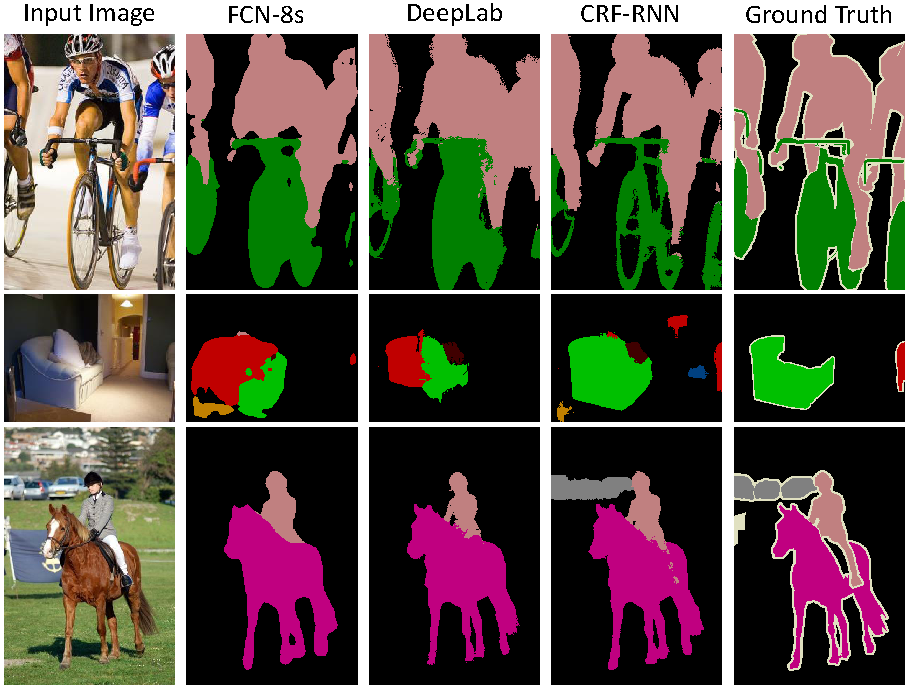
\includegraphics[width=0.85\textwidth]{../media/CRFasRNN.png}
\caption{\href{http://www.robots.ox.ac.uk/~szheng/CRFasRNN.html}{\color{blue}Zheng et al., CRF as RNN}}
\end{figure}
\end{frame}

\begin{frame}{Quality Assessment and Metrics}
Good, great, not bad, terrible?
\begin{figure}
\centering
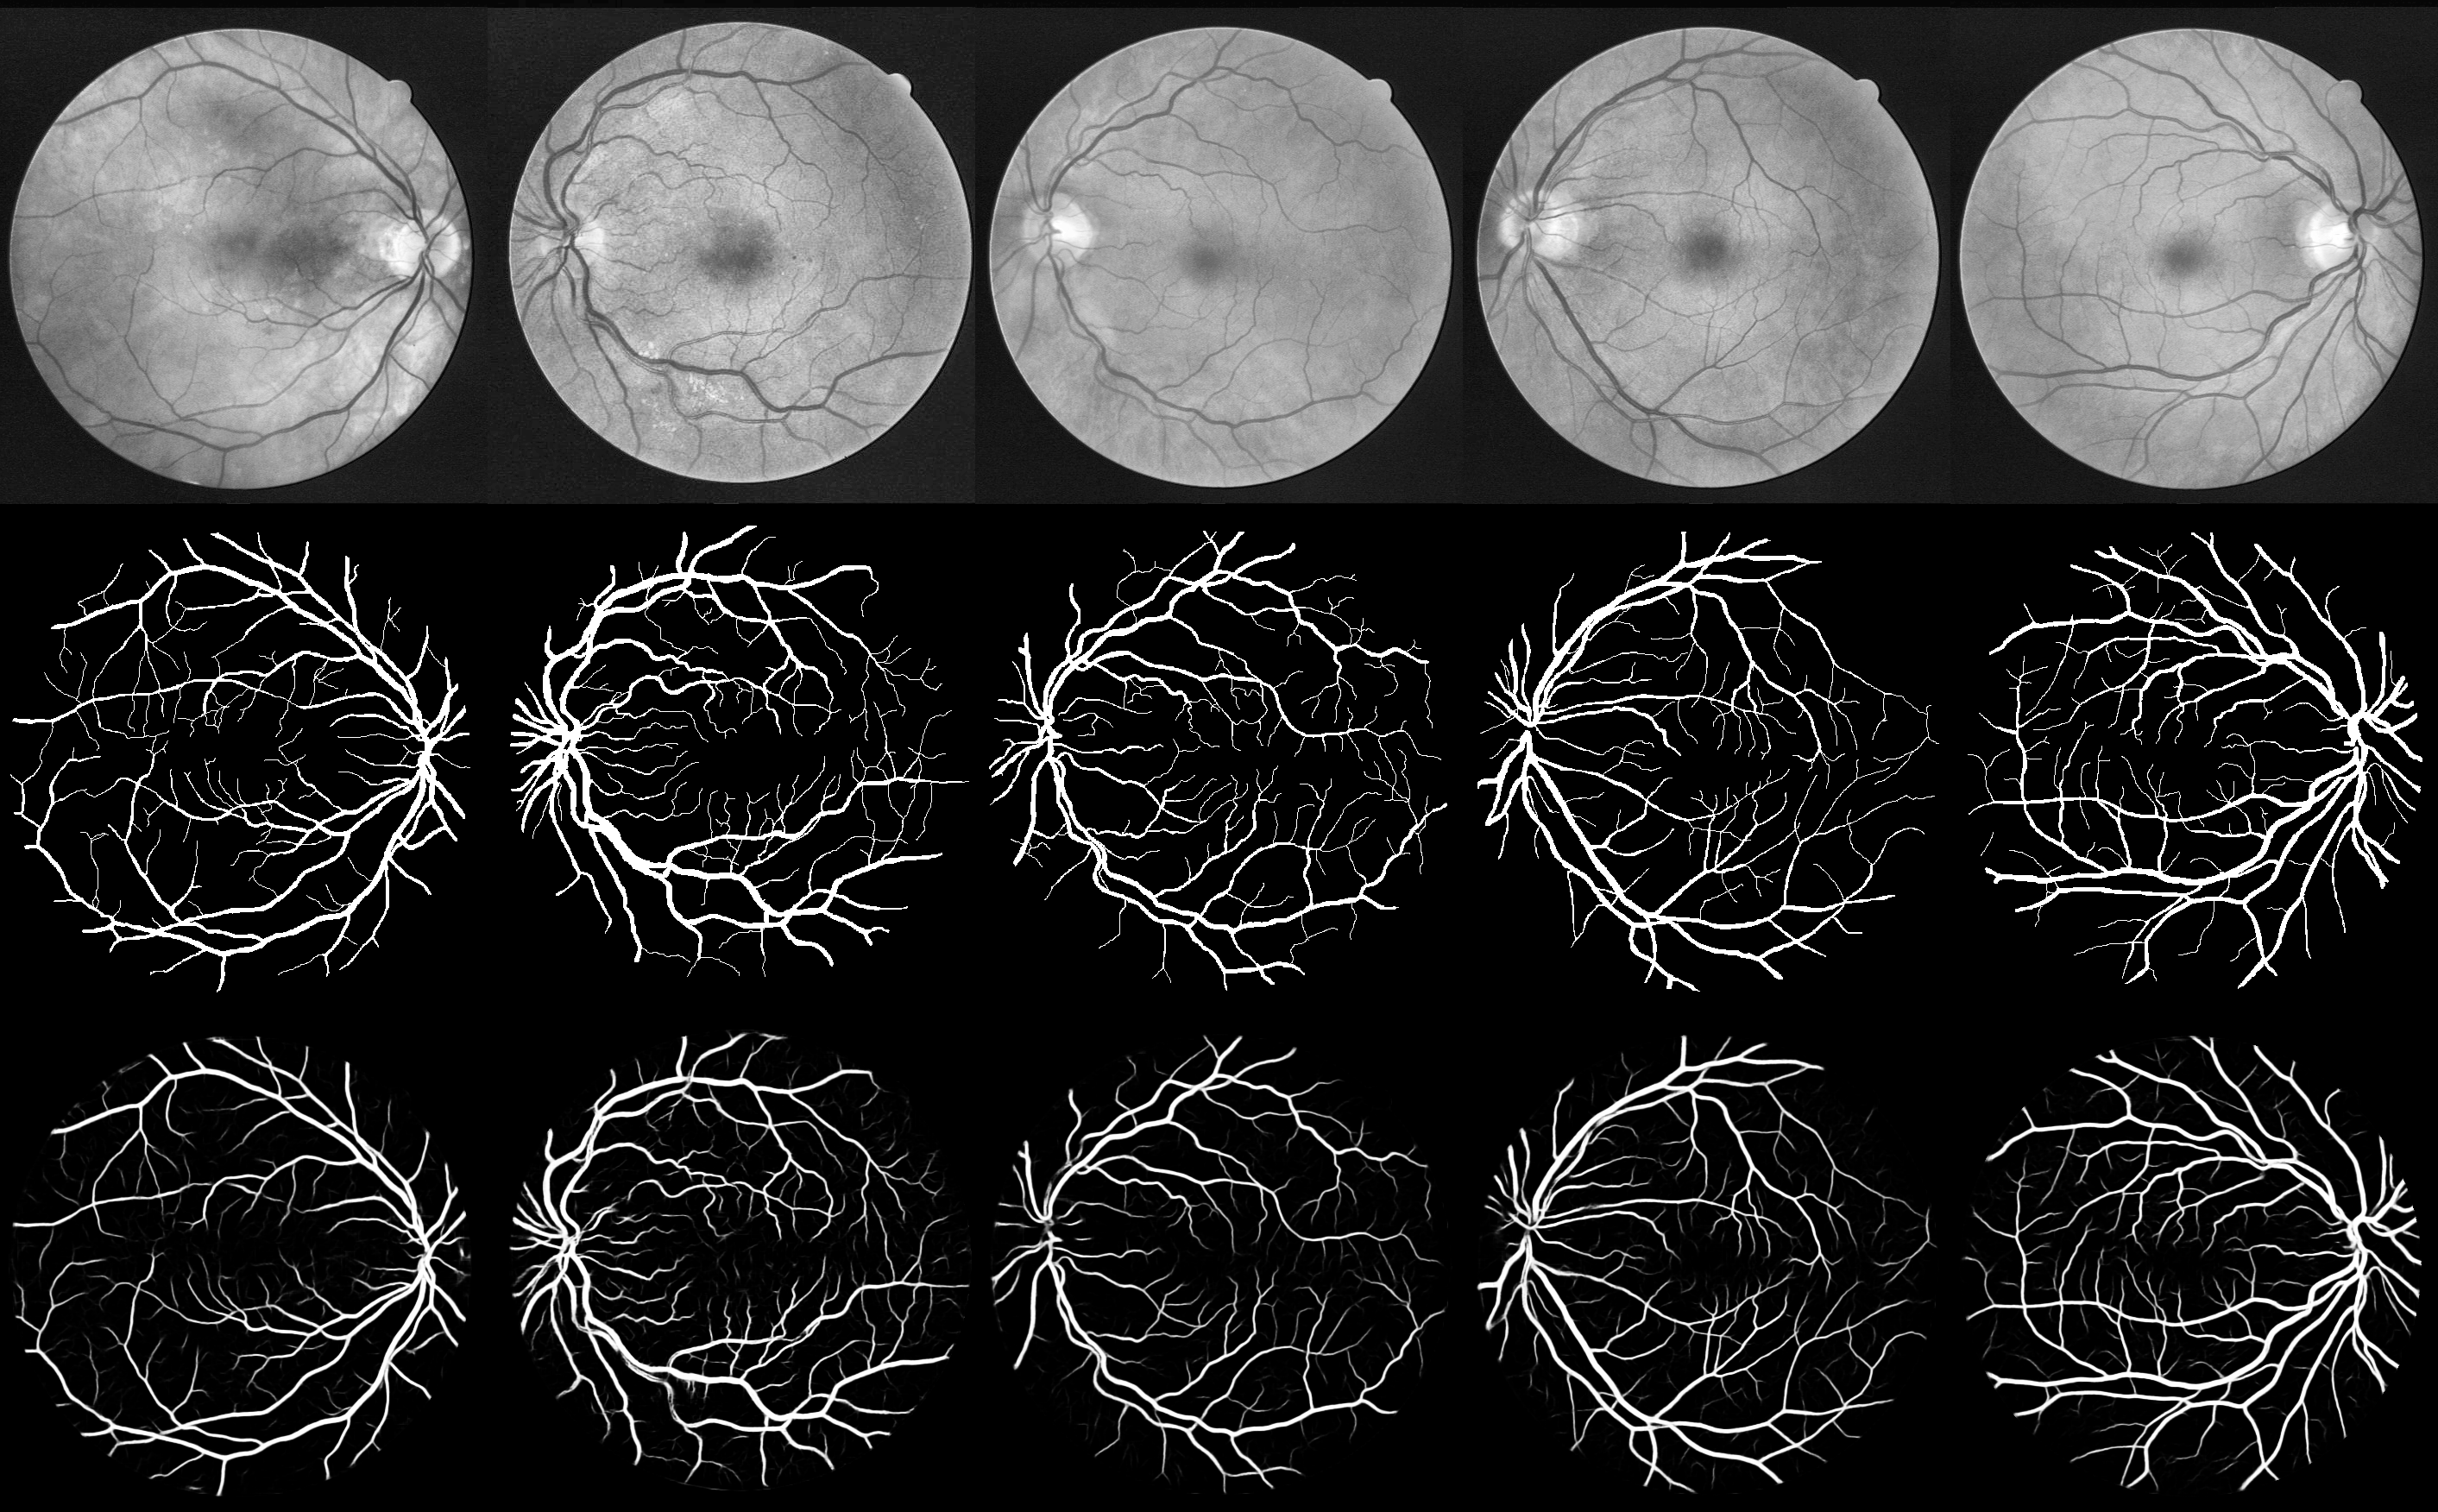
\includegraphics[width=0.8\textwidth]{../media/unet_retina_segmentation.png}
\caption{\href{https://arxiv.org/abs/1505.04597}{\color{blue}Ronneberger et al., U-Net: Biomedical Image Segmentation}}\end{figure}
\end{frame}

\begin{frame}{Quality Assessment and Metrics}
\begin{itemize}
\itemsep 1em
	\item<1->A common metric is \emph{mean average precision} (mAP)\footnote{see \href{http://host.robots.ox.ac.uk/pascal/VOC/pubs/everingham10.html\#abstract}{\color{blue}Everingham et al.} for more details}
	\begin{itemize}\setbeamertemplate{itemize items}[square]
		\item<1->For each class $c_i$, calculate average precision $ap_i = AP(c_i)$
		\item<2->Compute the mean over all $ap_i$ values calculated for each class
	\end{itemize}
	\item<2->Another common metric is \emph{intersection over union} (IoU)
	\begin{itemize}\setbeamertemplate{itemize items}[square]
		\item<1->Each bounding box (i.e. detection) is associated with a confidence (sometimes called \emph{rank})
		\item<2->Detections are assigned to ground truth objects and judged to be true/false positives by measuring overlap
		\item<3->To be considered a correct detection (i.e. true positive), the area of overlap $a_{ovl}$ between predicted bounding box $BB_p$ and the ground truth bounding box $BB_{gt}$ must exceed 0.5 according to 
	\end{itemize}
	\begin{equation}
		\centering
		\text{area}_{ovl} = \frac{\text{area}(\text{BB}_p \cap \text{BB}_{gt})}{\text{area}(\text{BB}_p \cup \text{BB}_{gt})}
	\end{equation}
	\begin{itemize}\setbeamertemplate{itemize items}[square]
		\item<4-> $\text{area}_{ovl}$ is often called \emph{intersection over union} (IoU)
	\end{itemize}
\end{itemize}
\end{frame}


\begin{frame}{Quality Assessment and Metrics}
\begin{figure}
\centering
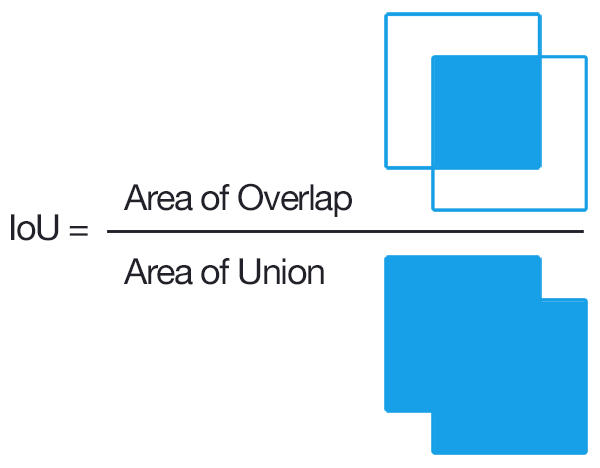
\includegraphics[width=0.8\textwidth]{../media/iou_equation.png}
\caption{\href{http://www.pyimagesearch.com/2016/11/07/intersection-over-union-iou-for-object-detection/}{\color{blue}Pyimagesearch: IoU for object detection}}
\end{figure}
\end{frame}


\begin{frame}{Quality Assessment and Metrics}
A few examples of IoU values and their associated configuration
\begin{figure}
\centering
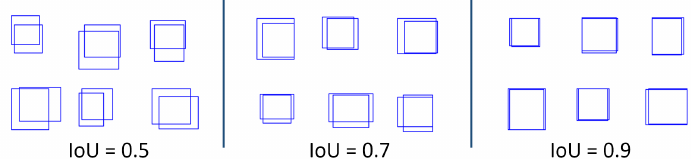
\includegraphics[width=\textwidth,keepaspectratio]{../media/iou-examples.png}
\caption{\href{https://leonardoaraujosantos.gitbooks.io/artificial-inteligence/content/object_localization_and_detection.html}{\color{blue}Leonardo Santos, Object Localization and Detection}}
\end{figure}
\end{frame}


\begin{frame}{Quality Assessment and Metrics}
\begin{figure}
\centering
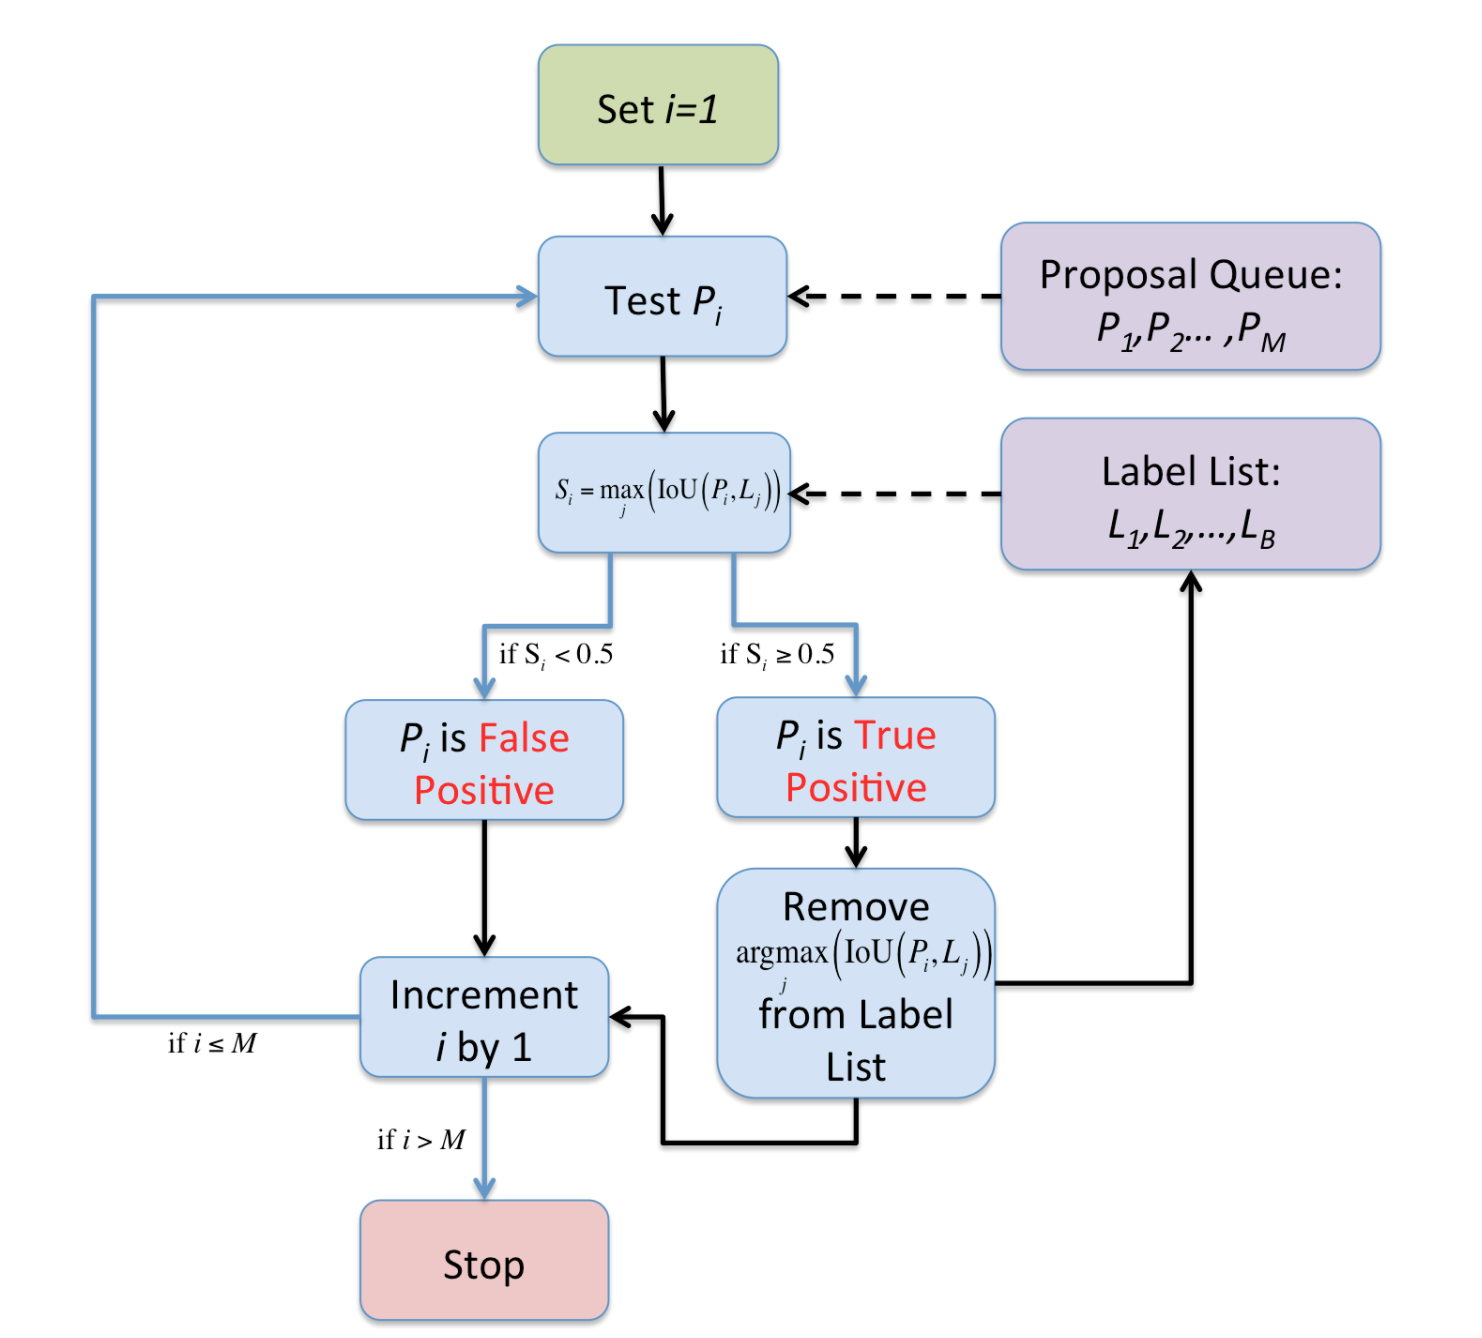
\includegraphics[width=0.7\textwidth]{../media/spacenet_perf_calc.png}
\caption{\href{https://medium.com/the-downlinq/the-spacenet-metric-612183cc2ddb}{\color{blue}The SpaceNet Metric}: A list of proposals is generated by the detection algorithm and compared to the ground truth in the list of labels}
\end{figure}
\end{frame}


\begin{frame}{Quality Assessment and Metrics}
\begin{itemize}
\itemsep 1em
	\item<1->A common metric used to evaluate segmentation performance is the percentage of pixels correctly labeled.  
	\item<2->Although, percentage correctly labeled can lead to situations where label all pixels as "pedestrian" class to maximize score on pedestrian class.
	\item<3->To rectify this, easy to modify assessment based on the intersection of the inferred segmentation and the ground truth divided by the union\footnote{Again, see \href{http://host.robots.ox.ac.uk/pascal/VOC/pubs/everingham10.html\#abstract}{\color{blue}Everingham et al.} for additional discussion}.  That is:
\end{itemize}
\begin{equation}
\centering
\text{seg.accuracy} = \frac{\text{true pos}}{\text{true pos}+\text{false neg}+\text{false pos}}
\end{equation}
\begin{itemize}
\itemsep 1em
	\item<4->Before machine learning, this was known as \href{https://en.wikipedia.org/wiki/Jaccard_index}{\color{blue}\emph{Jaccard Index}}
	\end{itemize}
\end{frame}

\section{PASCAL VOC2012 Leaderboard}
\begin{frame}{PASCAL VOC2012 Leaderboard}
\begin{figure}
\centering
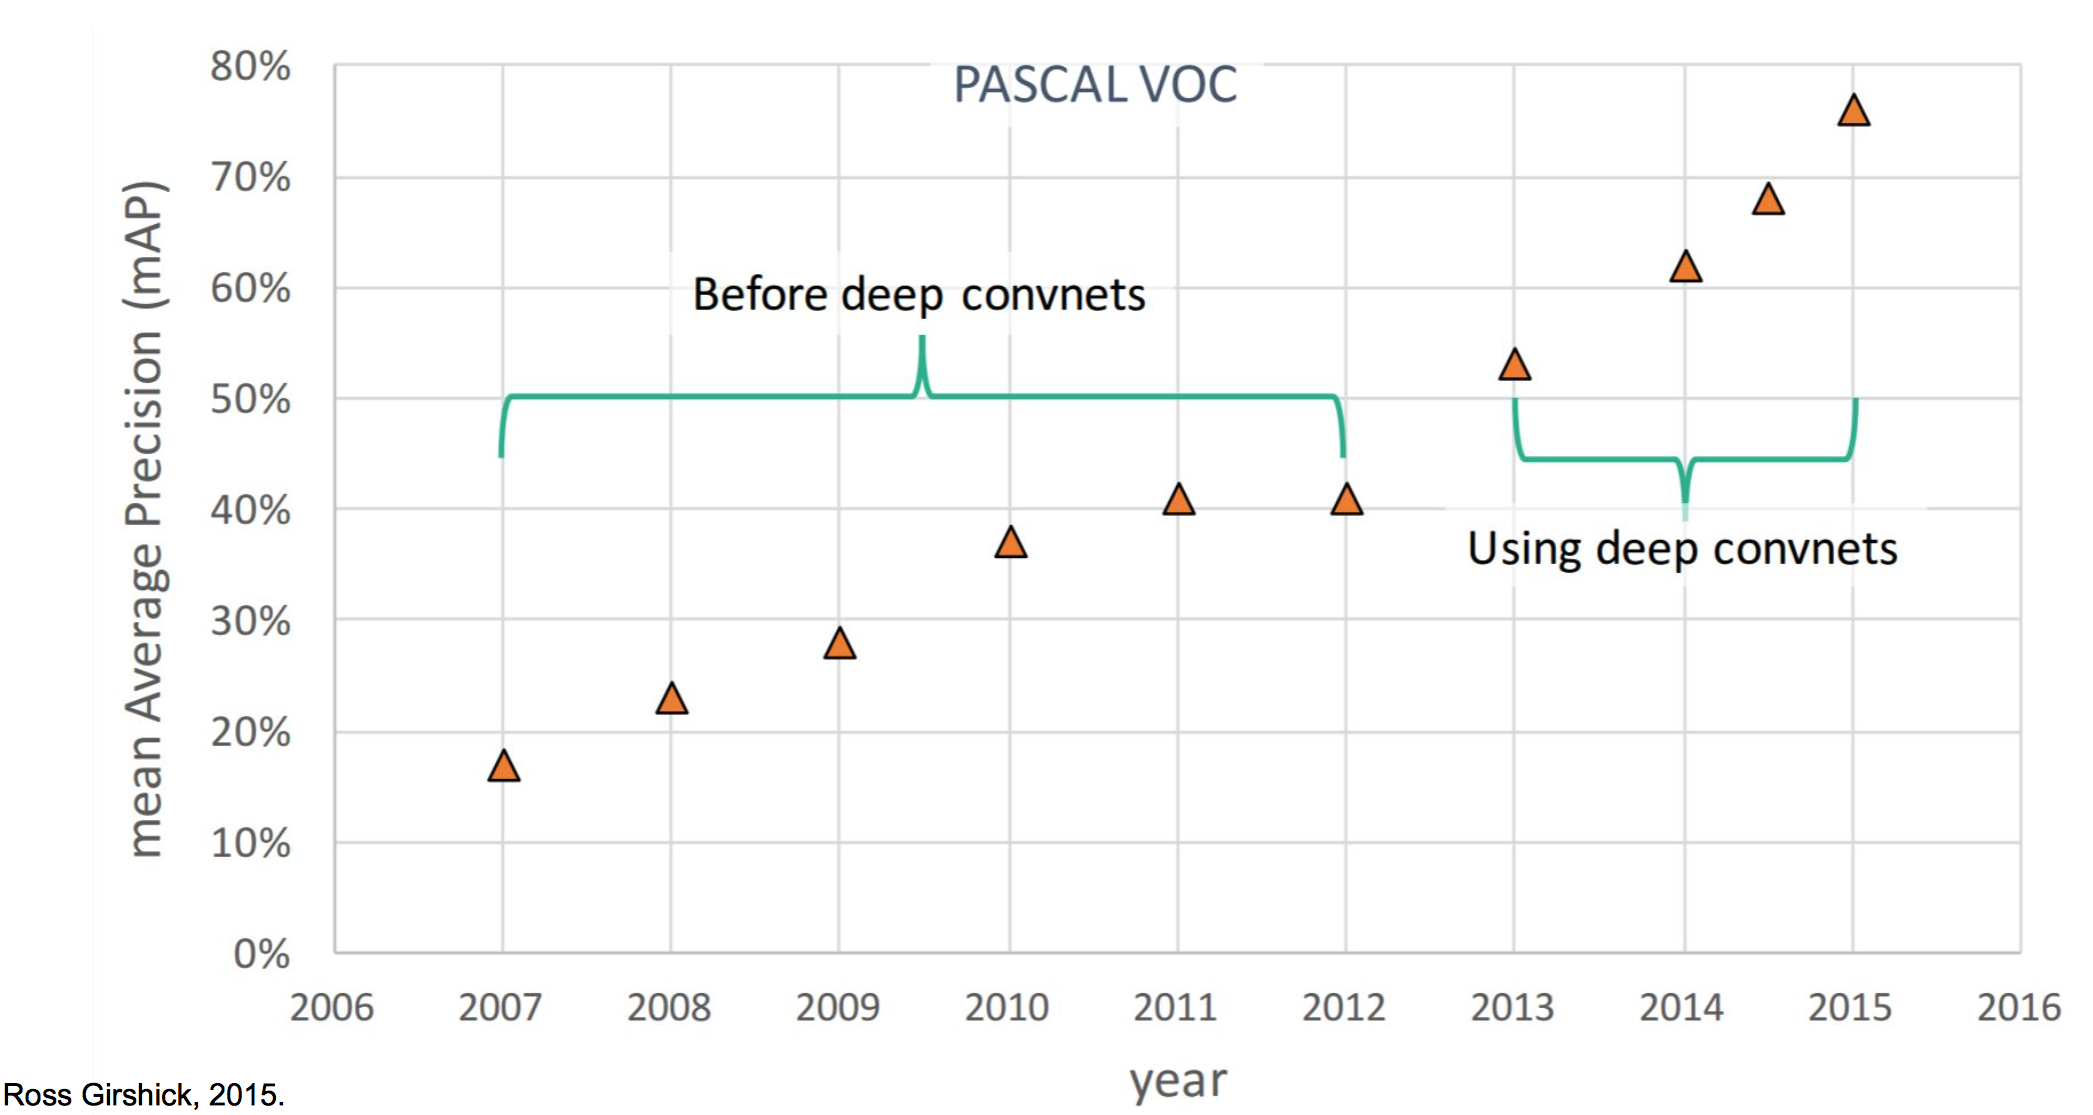
\includegraphics[width=\textwidth]{../media/dl_perf_pascal.png}
\caption{\href{http://host.robots.ox.ac.uk:8080/leaderboard/displaylb.php?challengeid=11&compid=6}{\color{blue}PASCAL VOC2012 segmentation leaderboard}.  As of 30-June-2017 top performance score of 86.3\% mPA }
\end{figure}
\end{frame}

\section{Exploring the R-CNN Family}

\begin{frame}{Early DL Detection and Segmentation}
\begin{itemize}
	\item<1->The early DL segmentation efforts looked a lot like traditional detection and segmentation workflows.
	\item<2->Although convolution neural networks had been around since late 1990s\footnote{\href{http://www.dengfanxin.cn/wp-content/uploads/2016/03/1998Lecun.pdf}{\color{blue}LeCun et al., Gradient-Based Learning Applied to Doc Recognition, 1998}}, it was not until CNNs won the \href{http://www.image-net.org}{\color{blue}ImageNet} competition in 2012 that \emph{deep learning} really took off.  
	\item<3->The winning ImageNet solution in 2012 was called \href{https://papers.nips.cc/paper/4824-imagenet-classification-with-deep-convolutional-neural-networks}{\color{blue}AlexNet} and was largely based on the original network architecture defined in LeCun's original paper.  
	\item<4->The \href{https://arxiv.org/abs/1312.6229}{\color{blue}Overfeat} (2013) solution was one of the first detection and localization strategies based on deep learning which leveraged the AlexNet success.
	\item<5->The Overfeat solution \enquote{\emph{explores the entire image by densely running the network at each location and at multiple scales}} via a sliding window approach.
\end{itemize}
\end{frame}

\begin{frame}{Early DL Solutions: The R-CNN Family}
\begin{itemize}
\itemsep 1em
	\item<1->The original \href{https://arxiv.org/abs/1311.2524}{\color{blue}R-CNN} approach combined aforementioned region proposal methods (i.e. \href{https://ivi.fnwi.uva.nl/isis/publications/bibtexbrowser.php?key=UijlingsIJCV2013\&bib=all.bib}{\color{blue}selective search}) with the \href{https://papers.nips.cc/paper/4824-imagenet-classification-with-deep-convolutional-neural-networks}{\color{blue}AlexNet} CNN in order to localize and segment objects 
	\item<2->Because region proposals are combined with CNNs, the method is referred to as 
	\enquote{\emph{\underline{\textbf{R}}egions with CNN features}} or \textbf{R}-CNN for short
	\item<3->Additionally, R-CNN was one of the first to propose \emph{transfer learning}: \enquote{\emph{when labeled training data is scarce, supervised pre-training for an auxiliary task followed by domain-specific fine-tuning yields a significant performance boost}}
\end{itemize}
\end{frame}

\begin{frame}{Early DL Solutions: The R-CNN Family}
\begin{figure}
        \centering
	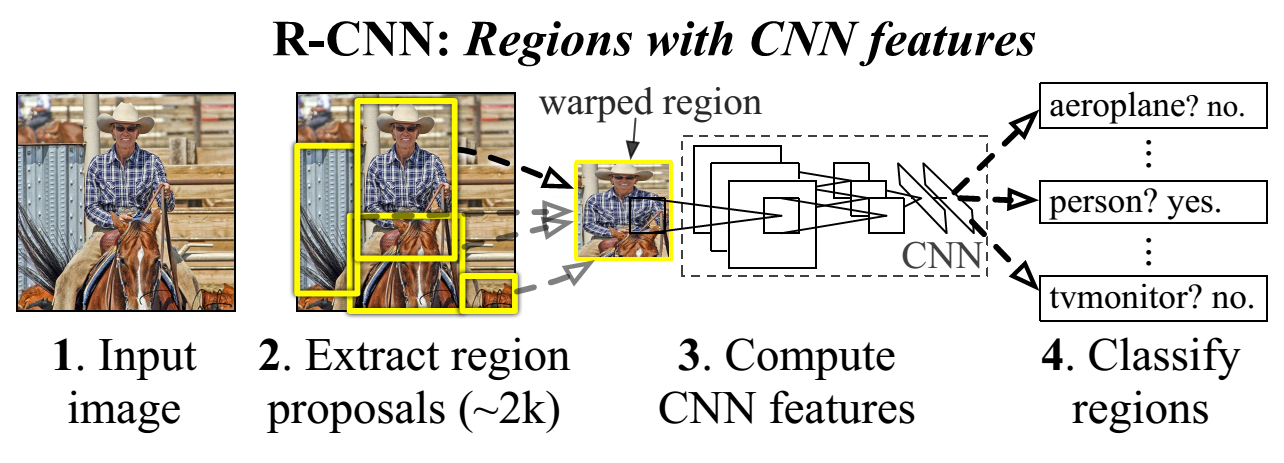
\includegraphics[width=\textwidth]{../media/r-cnn-approach.png}
	\caption{Girshick et al., Rich feature hierarchies, 2013}
\end{figure}
  \begin{itemize}
  	\item<1->identify potentially relevant content ($\approx$2k proposals/img)
	\item<2->for each proposed region: use CNN to generate feature vector
	\item<3->Use SVMs to classify each feature vector
	\item<4->Linear regression for bounding box offsets
  \end{itemize}
\end{frame}

\begin{frame}{Early DL Solutions: The R-CNN Family}
\begin{figure}
	\centering
	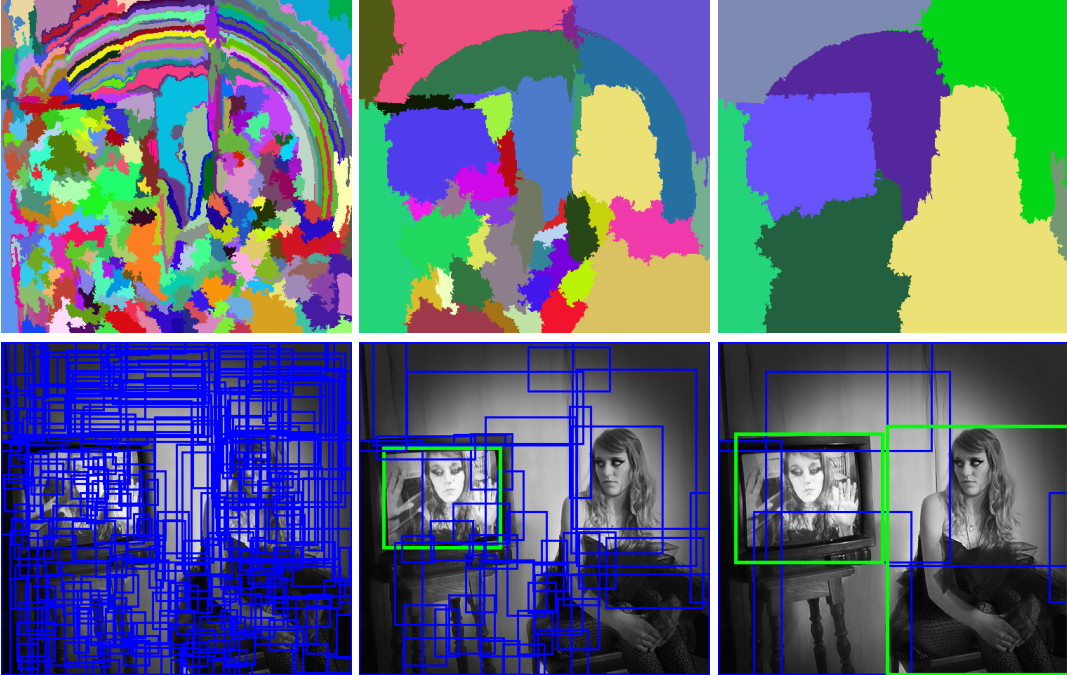
\includegraphics[width=0.8\textwidth,keepaspectratio]{../media/selective-search-example.png}
	\caption{Uijlings et al., Selective Search for Object Recognition, 2013}
\end{figure}
\end{frame}

\begin{frame}{Early DL Solutions: The R-CNN Family}
\begin{itemize} 
\itemsep 0.8em
	\item<1->Note that selective search produces \emph{many} region proposals 
	\item<2->Multiple stages must trained independently
	\begin{itemize}\setbeamertemplate{itemize items}[square]
		\item<1->Fine-tune network with softmax classifier (log loss)
		\item<2->Train post-hoc linear SVMs (hinge loss)
		\item<3->Train post-hoc bounding-box regressions (least squares)
	\end{itemize}
	\item<3->Training is slow (84h), takes a lot of disk space
	\item<4->R-CNN runtime roughly 47 seconds per image (\textcolor{red}{!})
	\item<5>Inference performance improved by spatial pyramid pooling networks SPPnets\footnote{\href{https://arxiv.org/abs/1406.4729}{\textcolor{blue}{He et al., Spatial Pyramid Pooling in Deep Convolutional Networks, 2014}}} which share convolutions between ROIs
	\item<6->Difficult training and slow inference motivates an update \ldots
	\item<7->For more details check out \href{http://mp7.watson.ibm.com/ICCV2015/ObjectDetectionICCV2015.html}{\textcolor{blue}{Girshick's ICCV 2015 tutorial}}
\end{itemize}
\end{frame}


\begin{frame}{The R-CNN Family: Fast R-CNN (2015)}
\begin{itemize}
\itemsep 0.8em
	\item<1->\href{https://arxiv.org/abs/1504.08083}{\color{blue}Fast R-CNN} is a combines stages 2 and 3 of R-CNN and is trained with multi-task loss (log loss and smooth L1 loss)
	\item<2->A Fast R-CNN network takes as input an image and a set of object proposals 
	\item<3->The network first processes the whole image with conv and pooling layers to produce a conv feature map.
	\item<4->For each object proposal an region of interest \emph{ROI} pooling layer extracts associated features from the conv map.
	\item<5->Each feature vector is fed into a fully connected (\emph{fc}) layer that finally branches into two sibling output layers:
	\begin{itemize}\setbeamertemplate{itemize items}[square]
		\item<1->A softmax layer producing classification labels
		\item<2->A linear layer producing bounding box positions
	\end{itemize}
	\item<6->Higher detection quality (mAP) than R-CNN and SPPnet
\end{itemize}
\end{frame}

\begin{frame}{The R-CNN Family: Fast R-CNN}
\begin{figure}
	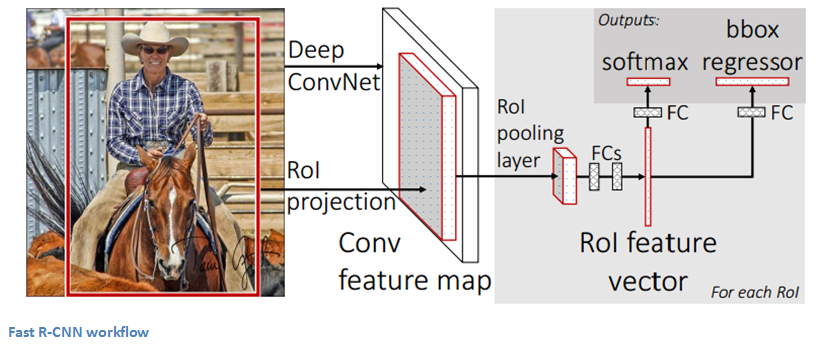
\includegraphics[width=\textwidth,keepaspectratio]{../media/fast-rcnn-diag.png}
	\caption{Girshick, Fast R-CNN, 2015}
\end{figure}
Fast R-CNN achieved the top results on PASCAL VOC12 at the time with an mAP of 68.4\% but still inference time is about 2.3 seconds per image (\textcolor{red}{2 sec/image for region proposal generation})
\end{frame}

\begin{frame}{The R-CNN Family: Fast R-CNN}
\begin{centering}
Can we do better \ldots?
\end{centering}
\end{frame}

\begin{frame}{The R-CNN Family: Fast\underline{\textbf{er}} R-CNN}
\begin{itemize}
\itemsep 0.6em
	\item<1->Fast R-CNN is still using independent region proposal stage.  
        \item<2->As you might guess, the Fast\textbf{er} R-CNN revision will introduce a Region Proposal Network (RPN) that shares full-image convolutional features with the detection network.
        \item<3->The RPN simultaneously predicts object bounds and \emph{objectness} scores at each position.
        \item<4->The RPN is trained end-to-end to generate high-quality region proposals which are used by Fast R-CNN 
        \item<5->The RPN and Fast R-CNN are merged into a single network by sharing their convolutional feature.  Using \enquote{\emph{attention}} mechanisms, the RPN component tells unified network where to look.
        \item<6->Multi-task training with 4 loss functions (obj/not obj, ROI bbox, classify, final obj bbox)
\end{itemize}
\end{frame}

\begin{frame}{The R-CNN Family: Fast\underline{\textbf{er}} R-CNN}
\begin{figure}
\centering
	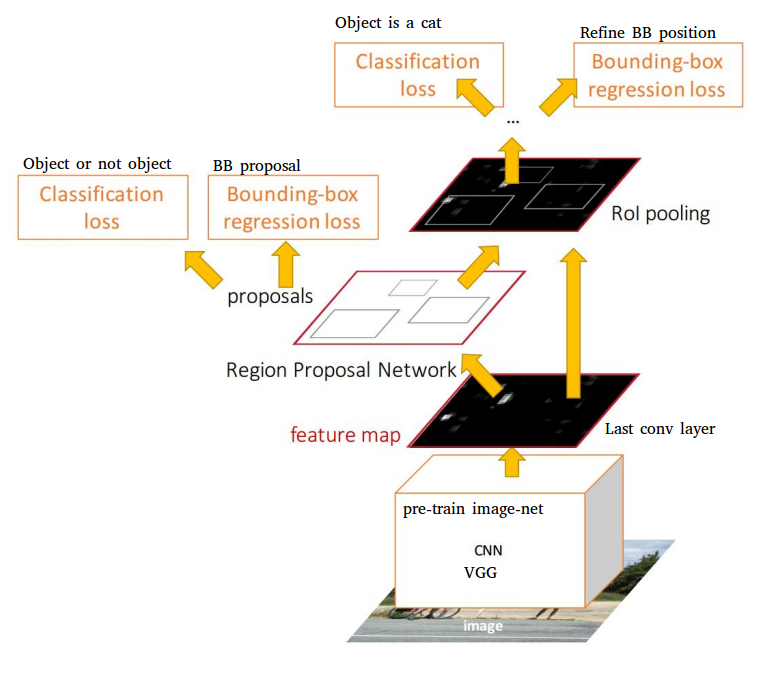
\includegraphics[width=0.7\textwidth,keepaspectratio]{../media/faster-rcnn-arch.png}
	\caption{\href{https://leonardoaraujosantos.gitbooks.io/artificial-inteligence/content/object_localization_and_detection.html}{\color{blue}Leonardo Santos, Object Localization and Detection}}
\end{figure}
\end{frame}

\begin{frame}{The R-CNN Family: Fast\underline{\textbf{er}} R-CNN}
\begin{itemize}
\itemsep 1em
	\item<1->Fast\textbf{er} R-CNN based on \href{https://arxiv.org/abs/1409.1556}{\color{blue}VGG-16} model, the detection system has a frame rate of 5 fps on a GPU (i.e. 200 ms)
	\item<2->Fast\textbf{er} R-CNN generates about 300 proposals per image
	\item<3->Fast\textbf{er} R-CNN, at the time, achieved state-of-the-art object detection accuracy on PASCAL \href{http://host.robots.ox.ac.uk/pascal/VOC/voc2012/}{\color{blue}VOC12} and \href{http://mscoco.org}{\color{blue}MS COCO} datasets
	\item<4->All codes for Fast\textbf{er} R-CNN are available on GitHub \href{https://github.com/rbgirshick/py-faster-rcnn}{\color{blue}here}

\end{itemize}
\end{frame}

\begin{frame}{The R-CNN Family: Fast\underline{\textbf{er}} R-CNN}
\begin{centering}
Can we do \emph{even} better\underline{\textbf{er}} \ldots?
\end{centering}
\end{frame}

\begin{frame}{The R-CNN Family: Mask R-CNN}
\begin{itemize}
\itemsep 1em
	\item<1->At the time of writing, \href{}{\color{blue}Mask R-CNN} (2017) is gaining significant popularity. 
	\item<2->As the name implies, Mask R-CNN is an R-CNN derivative combining the best of \href{https://arxiv.org/abs/1612.03144}{\color{blue}Feature Pyramid Pooling} (FPN), \href{https://arxiv.org/abs/1411.4038}{\color{blue}Fully Convolutional Networks} (FCNs), and \href{https://arxiv.org/abs/1512.03385}{\color{blue}Residual networks} all together under the Fast\textbf{er} R-CNN architecture.
	\item<3->Furthermore, Mask R-CNN extends Fast\textbf{er} R-CNN by adding an additional branch for predicting an object mask (i.e. pixel segmentation) in parallel with the existing branch for bounding box recognition.  
	\item<4->Mask R-CNN achieves top marks in all three tracks of the \href{http://mscoco.org}{\color{blue}COCO} suite of challenges, including \href{http://mscoco.org/dataset/\#detections-challenge2016}{\color{blue}instance segmentation}, bounding-box \href{http://mscoco.org/dataset/\#detections-challenge2016}{\color{blue}object detection}, and person \href{http://mscoco.org/dataset/\#keypoints-challenge2016}{\color{blue}keypoint detection}.  
\end{itemize}
\end{frame}

\begin{frame}{The R-CNN Family: Mask R-CNN}
Results on COCO test images using ResNet-101-FPN at 5 fps. 
\begin{figure}
\centering
	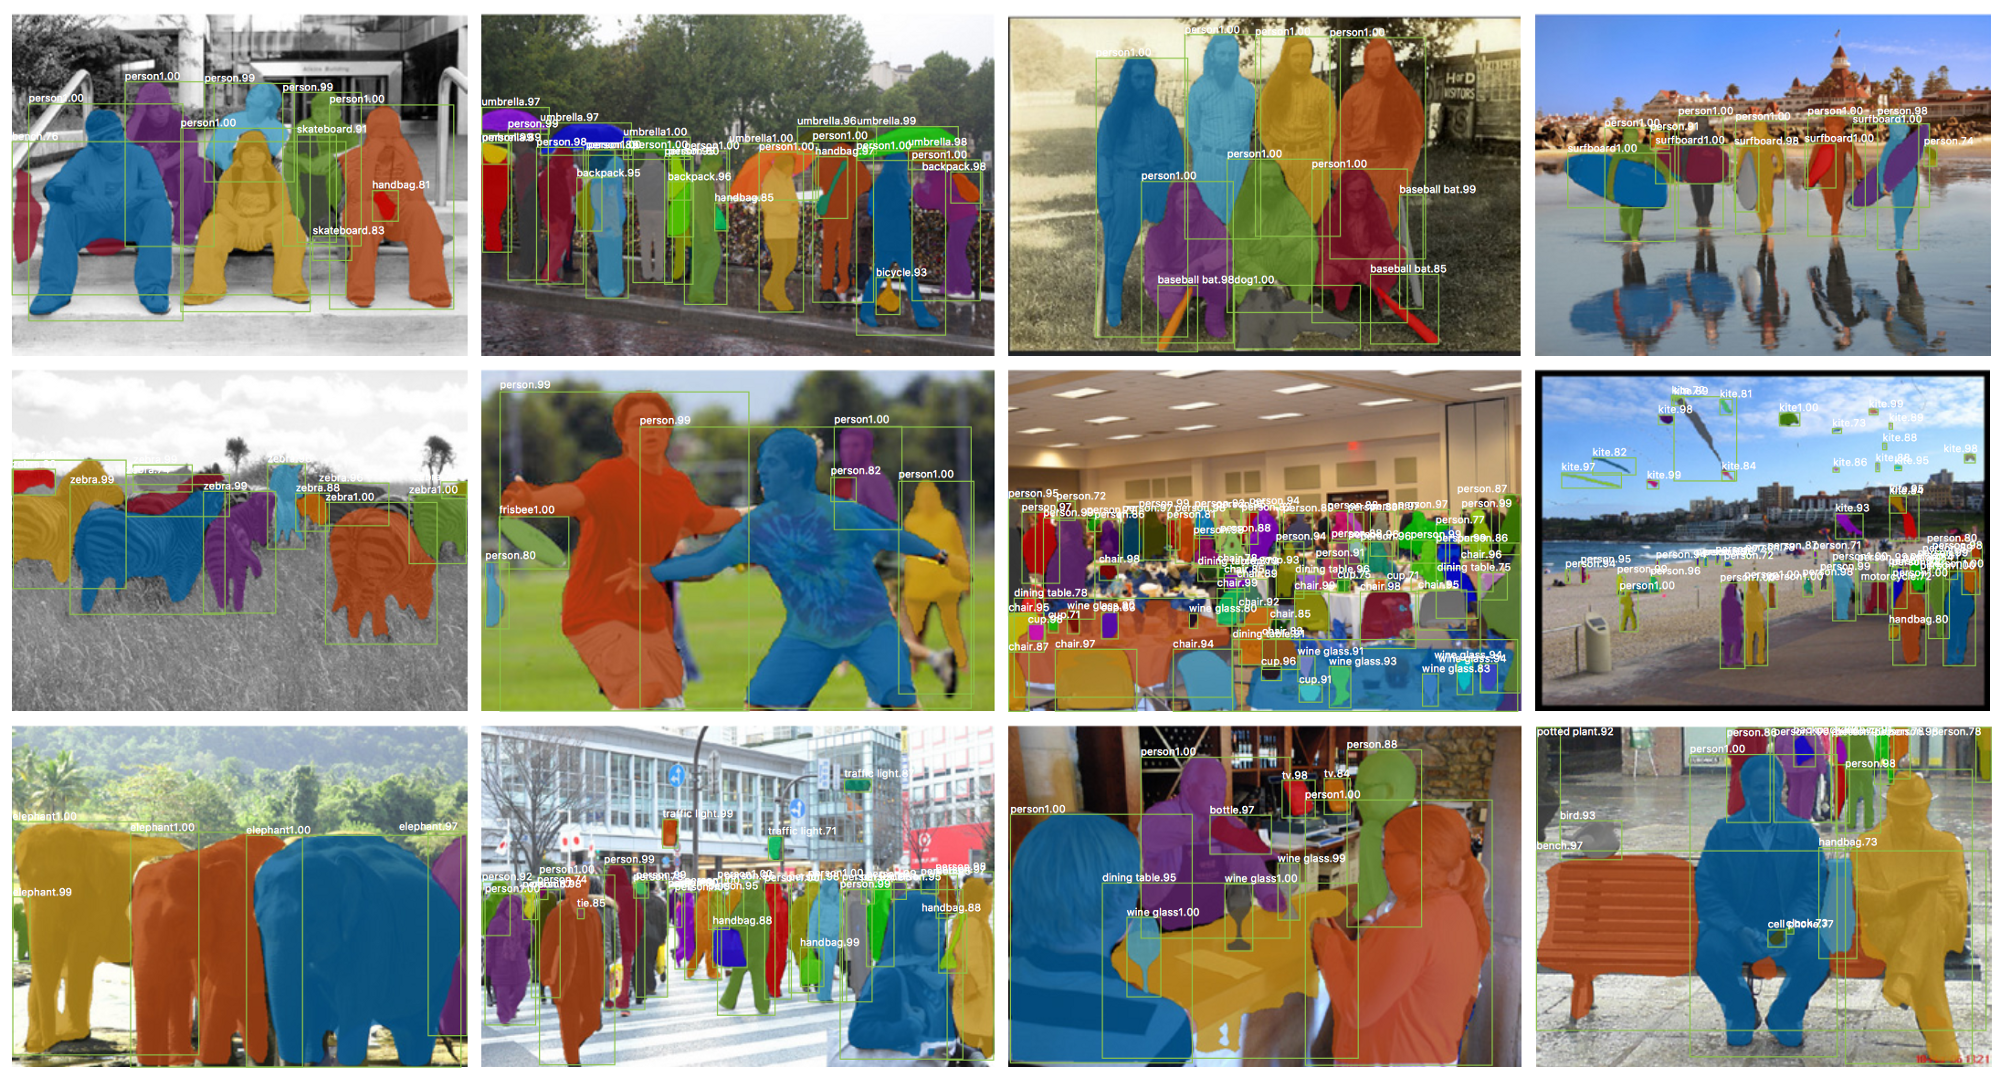
\includegraphics[width=\textwidth,keepaspectratio]{../media/mask-rcnn-examples.png}
	\caption{He et al., \href{https://arxiv.org/abs/1703.06870}{\color{blue}Mask R-CNN}, 2017}
\end{figure}
\end{frame}

\section{A Thriving Ecosystem}
\begin{frame}{Wrapping up: A Thriving Ecosystem}
\begin{itemize}
\itemsep 1em
	\item<1->The R-CNN family history is a classic example of traditional computer vision approaches incrementally adopting convolution neural networks to iteratively improve performance and expand algorithm capabilities 
	\item<2->However, the R-CNN variety architecture is only one of \emph{many} different approaches for object detection and segmentation
	\item<3->Other key CNN based contributions include:
	\begin{itemize}\setbeamertemplate{itemize items}[square]
		\item<1>\href{https://arxiv.org/abs/1411.4038}{\color{blue}Fully Convolutional Networks} (2014)  
		\item<2>\href{https://arxiv.org/abs/1505.04366}{\color{blue}Learning Deconvolution Networks} (2015)
		\item<3>\href{https://arxiv.org/abs/1512.02325}{\color{blue}Single-Shot Deep MultiBox} (2015)
		\item<4>\href{https://arxiv.org/abs/1511.00561}{\color{blue}SegNet: an Encoder-Decoder Architecture} (2015)
		\item<5>\href{https://arxiv.org/abs/1606.00915}{\color{blue}DeepLab: Atrous Convolutions and CRFs} (2016)
		\item<6>The \href{https://research.fb.com/category/facebook-ai-research-fair/}{\color{blue}FB} suite: \href{https://arxiv.org/abs/1506.06204}{\color{blue}DeepMask}, \href{https://arxiv.org/abs/1603.08695}{\color{blue}SharpMask}, \& \href{https://arxiv.org/abs/1604.02135}{\color{blue}MultiPath} (2016)
		\item<7>\href{https://github.com/tensorflow/models/tree/master/object_detection}{\color{blue}TensorFlow Object Detection API} (2017)
	\end{itemize}
\end{itemize}
\end{frame}

\section{The Atlas}
\begin{frame}[fragile]{Detection and Segmentation Atlas}
\fontsize{8}{12}\selectfont There are too many outstanding contributions to cover in a single deck.  Here is a brief high-level overview intended to provide broader context and help guide additional exploration.
\begin{figure}
\Wider[3.8em]{
\begin{center}
\resizebox{\textwidth}{!}{
\begin{tikzpicture} [
    nodes={
      text height=.7em,
      text depth=.2em,
      draw=black!20,
      %draw=none,
      thick, 
      fill=none, 
      font=\footnotesize,
    },
    >=stealth',
    rounded corners,
    semithick,
    tree layout
 ] 
   \node[] (A) [] {\href{http://www.dengfanxin.cn/wp-content/uploads/2016/03/1998Lecun.pdf}{LeNet (1998)}};
   \node[] (B) [] {\href{https://arxiv.org/abs/1003.0358}{Big Simple Nets (2010)}};
   \node[] (C) [] {\href{https://papers.nips.cc/paper/4824-imagenet-classification-with-deep-convolutional-neural-networks}{AlexNet (2012)}};
   
   \node[] (D) [] {\href{http://www.matthewzeiler.com/pubs/iccv2011/iccv2011.pdf}{Adaptive Deconv Nets (2011)}};
   \node[] (E) [] {\href{https://arxiv.org/abs/1311.2901}{Understanding Conv Nets (2013)}};
   \node[] (F) [] {\href{https://arxiv.org/abs/1505.04366}{Learning Deconv Nets (2015)}};
   \node[] (G) [] {\href{https://arxiv.org/abs/1511.07356}{Recombinator Nets (2015)}};
   \node[] (H) [] {\href{https://arxiv.org/abs/1505.04597}{U-Networks (2015)}};
   
   \node[](I)[]{\href{https://arxiv.org/abs/1409.1556}{VGG (2014)}};
   
   \node[](J)[]{\href{https://arxiv.org/abs/1511.00561}{SegNet (2015)}};
   \node[](U)[]{\href{https://arxiv.org/abs/1506.02142}{Dropout Bayes (2015)}};
   \node[](V)[]{\href{https://arxiv.org/abs/1511.02680}{Bayes SegNet (2015)}};
   
   \node[](K)[] {\href{https://arxiv.org/abs/1606.00915}{DeepLab (2016)}};
   \node[](P)[]{\href{https://arxiv.org/abs/1706.05587}{Rethinking Atrous (2017)}};
   \node[](Q)[]{\href{http://homepages.inf.ed.ac.uk/csutton/publications/crftutv2.pdf}{CRFs (2012)}};
   \node[](R)[]{\href{https://arxiv.org/abs/1412.6071}{Frac Max-Pooling (2014)}};
   \node[](S)[]{\href{https://arxiv.org/abs/1512.09194}{Kroneker Layer (2015)}};
   \node[](T)[]{\href{https://arxiv.org/abs/1511.07122}{Dilated Conv (2015)}};
   
   
   \node[](L)[]{\href{https://arxiv.org/abs/1506.06204}{DeepMask (2015)}};
   \node[](M)[]{\href{https://arxiv.org/abs/1603.08695}{SharpMask (2016)}};
   \node[](N)[]{\href{https://arxiv.org/abs/1604.02135}{MultiPath (2016)}};
   \node[](O)[]{\href{https://arxiv.org/abs/1612.03144}{FPN (2016)}};

   
   % R-CNN branch
   \node[](AA)[]{\href{https://arxiv.org/abs/1312.6229}{Overfeat (2013)}};
   \node[](BB)[]{\href{https://arxiv.org/abs/1311.2524}{R-CNN (2013)}};
   \node[](CC)[]{\href{https://arxiv.org/abs/1504.08083}{Fast R-CNN (2015)}};
   \node[](DD)[]{\href{https://arxiv.org/abs/1506.01497}{Fast\textbf{er} R-CNN (2015)}};
   \node[](EE)[]{\href{https://arxiv.org/abs/1605.06409}{R-FCN (2016)}};
   \node[](FF)[]{\href{https://arxiv.org/abs/1703.06870}{Mask R-CNN (2017)}};
   \node[](GG)[]{\href{https://arxiv.org/abs/1704.05776}{RRC (2017)}};
   
   % GoogleNet, ResNet and all that
   \node[](HH)[]{\href{https://arxiv.org/abs/1409.4842}{GoogleNet$_{V1}$ (2014)}};
   \node[](II)[]{\href{https://arxiv.org/abs/1512.00567}{GoogleNet$_{V2,V3}$ (2015)}};
   \node[](JJ)[]{\href{https://arxiv.org/abs/1512.03385}{ResNet (2015)}};
   \node[](KK)[]{\href{https://arxiv.org/abs/1602.07261}{GoogleNet$_{V4}$ (2016)}};
   \node[](LL)[]{\href{https://arxiv.org/abs/1611.05431}{ResNeXt (2016)}};
   
   % bounding box regression, google object detection, etc
   \node[](MM)[]{\href{https://papers.nips.cc/paper/5207-deep-neural-networks-for-object-detection}{Deep MultiBox (2013)}};
   \node[](NN)[]{\href{https://arxiv.org/abs/1412.1441}{Multi-scale MultiBox (2014)}};
   \node[](OO)[]{\href{https://arxiv.org/abs/1512.02325}{Single-Shot MultiBox (2015)}};
   \node[](PP)[]{\href{https://arxiv.org/abs/1611.10012}{Speed/Acc Trade-offs (2016)}};
   \node[](QQ)[]{\href{https://arxiv.org/abs/1612.02297}{Spatially Adaptive Nets (2016)}};
   \node[](RR)[]{\href{https://arxiv.org/abs/1612.06851}{Beyond Skip Conns (2016)}};
   \node[](SS)[]{\href{https://arxiv.org/abs/1704.04861}{MobileNets (2017)}};
   \node[](TT)[]{\href{https://github.com/tensorflow/models/tree/master/object_detection}{TF Object Detection API (2017)}};
   
   % yolo & fcn
   \node[](UU)[]{\href{https://arxiv.org/abs/1411.4038}{FCNs (2014)}};
   \node[](VV)[]{\href{https://arxiv.org/abs/1506.02640}{YOLO (2015)}};
      
  \graph [
    tree layout,
    level distance=1cm,
    sibling sep=.5em,
    sibling distance=1cm,
    use existing nodes
  ] {
  
  (A) -> (D) -> (E) -> (F) -> (G) -> (H);  
  (C) -> (E);
  (C) -> (I);
  (I) -> (J);
  (I) -> (R);
  
  % crfs to deep lab
  (Q) -> (K);
  (R) -> (S);
  (S) -> (T);
  (T)-> (K);
  
  (I) -> (L);
  (A) -> (B) -> (C);
  
  % unet to segnet
  (H) <->[dashed,color=black!50] (J);
  
  %deepmask to sharp mask to multipath to FPN
  (L)->(M);
  (M)->(N);
  (N)->(O);
  
  % Deep Lab branch
  (K)->(P);
  
  %segnet branch
  (J)->(U);
  (U)->(V);
  
  %R-CNN branch
  (C) -> (AA) -> (BB) -> (CC) -> (DD) -> (EE) -> (FF) -> (GG);
  
   % fcn and yolo connections
  (UU) -> (VV);
  %(I) ->(UU);
  (C) ->(UU);
  (HH) <->[dashed,color=black!50] (UU);
  %(II)    <->[dashed,color=black!50] (UU);
  %(JJ) <-> [dashed,color=black!50](UU);
  %(KK) <- (UU);
  
  %(CC) -> (UU)
  
  %(UU)->(EE);
  
  % FPN to mask r-cnn
  (O) ->[dashed,color=black!50] (FF);
  
  % mask r-cnn to resnet and resNeXt
  %(JJ)<->[dashed](FF);
  (LL)<-[dashed,color=black!50](FF);
  
  % googlenet resnet branch
  (C) -> (HH) -> (II) -> (JJ) -> (KK) -> (LL);
  
  % google multibox and object detection
  (C) -> (MM) -> (NN) -> (OO) -> (PP) -> (QQ) -> (RR) -> (SS) -> (TT);
  
  %VGG to R-CNN
  %(C)->(BB);
  
  %
  (FF)->[dashed,color=black!50](RR);
  (JJ)->[dashed,color=black!50](PP);
  
}; %graph
\end{tikzpicture}

} %resize
\end{center}
} %wider
\caption{Nodes are hyperlinks to the associated \href{https://arxiv.org}{\color{blue}arXiv.org} papers.  }
\end{figure}
\end{frame}

\section{Public Datasets}
\begin{frame}{Public Datasets}
\begin{tabular}{lccc}
	 Inria Aerial Image Labeling \dotfill & 2017 & \href{https://hal.inria.fr/hal-01468452/document}{\color{blue}paper} & \href{https://project.inria.fr/aerialimagelabeling/}{\color{blue}data} \\
	 DAVIS Challenge \dotfill & 2017 & \href{https://arxiv.org/abs/1704.00675}{\color{blue}paper} & \href{http://davischallenge.org/challenge2017/index.html}{\color{blue}data} \\
	 Mapillary Vistas \dotfill & 2017 & \href{http://blog.mapillary.com/product/2017/05/03/mapillary-vistas-dataset.html}{\color{blue}paper} & \href{https://www.mapillary.com/dataset/vistas?lat=20\&lng=0\&z=1.5}{\color{blue}data} \\
	 ADE20K \dotfill & 2016 & \href{https://arxiv.org/abs/1608.05442}{\color{blue}paper} & \href{http://groups.csail.mit.edu/vision/datasets/ADE20K/}{\color{blue}data}\\
	 SYNTHIA \dotfill & 2016 & \href{http://www.cv-foundation.org/openaccess/content_cvpr_2016/papers/Ros_The_SYNTHIA_Dataset_CVPR_2016_paper.pdf}{\color{blue}paper} & \href{http://synthia-dataset.net/dataset/}{\color{blue}data}\\
	 SpaceNet \dotfill & 2016 & N/A & \href{https://aws.amazon.com/public-datasets/spacenet/}{\color{blue}data}\\
	 Playing for Data \dotfill & 2016 & \href{https://arxiv.org/abs/1608.02192}{\color{blue}paper} & \href{https://download.visinf.tu-darmstadt.de/data/from_games/}{\color{blue}data}\\
	 SUN RGB-D \dotfill & 2015 & \href{http://rgbd.cs.princeton.edu/paper.pdf}{\color{blue}paper} & \href{http://rgbd.cs.princeton.edu}{\color{blue}data} \\
	 Cityscapes\dotfill & 2015 & \href{https://arxiv.org/abs/1604.01685}{\color{blue}paper} & \href{https://www.cityscapes-dataset.com}{\color{blue}data}\\
	 Common Objects in Context (COCO) & 2014 & \href{https://arxiv.org/abs/1405.0312}{\color{blue}paper} & \href{http://mscoco.org/dataset/\#overview}{\color{blue}data}\\
	 Oxford RoboCar Dataset \dotfill & 2014 & \href{http://robotcar-dataset.robots.ox.ac.uk/images/robotcar_ijrr.pdf}{\color{blue}paper} & \href{http://robotcar-dataset.robots.ox.ac.uk/datasets/}{\color{blue}data}\\
	 KITTI Vision Benchmark Suite\dotfill & 2012 & \href{http://citeseerx.ist.psu.edu/viewdoc/download?doi=10.1.1.296.7277\&rep=rep1\&type=pdf}{\color{blue}paper} & \href{http://www.cvlibs.net/datasets/kitti/}{\color{blue}data}\\
	Visual Object Classes 2012 (VOC12)\dotfill & 2012 & [\href{http://host.robots.ox.ac.uk/pascal/VOC/pubs/everingham10.html\#abstract}{\color{blue}1}][\href{http://host.robots.ox.ac.uk/pascal/VOC/pubs/everingham15.html\#abstract}{\color{blue}2}] & \href{http://host.robots.ox.ac.uk/pascal/VOC/voc2012/}{\color{blue}data} \\
	NYU Depth Dataset V2 \dotfill & 2012 & \href{http://cs.nyu.edu/~silberman/papers/indoor_seg_support.pdf}{\color{blue}paper} & \href{http://cs.nyu.edu/~silberman/datasets/nyu_depth_v2.html}{\color{blue}data} \\
	Caltech Pedestrian Detection Benchmark\dotfill & 2009 & [\href{http://www.vision.caltech.edu/Image_Datasets/CaltechPedestrians/files/CVPR09pedestrians.pdf}{\color{blue}1}][\href{http://www.vision.caltech.edu/Image_Datasets/CaltechPedestrians/files/PAMI12pedestrians.pdf}{\color{blue}2}] & \href{http://www.vision.caltech.edu/Image_Datasets/CaltechPedestrians/index.html}{\color{blue}data} \\
	CamVid: Motion-based Segmentation\dotfill & 2008 &\href{http://citeseerx.ist.psu.edu/viewdoc/download?doi=10.1.1.480.7333\&rep=rep1\&type=pdf}{\color{blue}paper} & \href{http://mi.eng.cam.ac.uk/research/projects/VideoRec/CamVid/}{\color{blue}data} \\	
\end{tabular}
\end{frame}

\end{document}
